% =============================================================================
% GRAIL Reference Guide
% =============================================================================
% Public technical reference for GRAIL.
% Compile from this directory:
%   pdflatex grail_reference_guide  (twice for ToC + cross-refs)
% Builds independently from the supplied library and technical sources.
% =============================================================================

\documentclass[11pt]{article}
\usepackage[margin=1in]{geometry}
\usepackage{amsmath,amssymb,amsthm}
\usepackage[T1]{fontenc}
\usepackage{lmodern}
\usepackage[colorlinks=true,linkcolor=blue,citecolor=blue,urlcolor=blue]{hyperref}
\usepackage[numbers,sort&compress]{natbib}
\usepackage{enumitem}
\usepackage{booktabs}
\usepackage{graphicx}
\usepackage{xcolor}
\usepackage{titlesec}
\usepackage{listings}
\usepackage{tikz}
\usetikzlibrary{arrows.meta,positioning,calc,shapes.geometric,decorations.pathreplacing,backgrounds}
\usepackage{pgfplots}
\pgfplotsset{compat=1.18}
\usepgfplotslibrary{groupplots}
\usepackage{longtable}

\setlist{nosep}

\titlespacing*{\section}{0pt}{14pt}{6pt}
\titlespacing*{\subsection}{0pt}{10pt}{4pt}
\titlespacing*{\subsubsection}{0pt}{8pt}{3pt}

% Math shorthand.
\newcommand{\Lop}{\Lambda}
\newcommand{\Lstar}{\Lambda^{*}}
\newcommand{\Tcyc}{\mathcal{T}}
\newcommand{\Trt}{\Tcyc_{\mathrm{RT}}}
\newcommand{\Tse}{\Tcyc_{\mathrm{SE}}}
\newcommand{\dT}{\delta\Tcyc}
\newcommand{\Jbar}{\bar{J}}
\newcommand{\Bnu}{B_{\nu}}
\newcommand{\half}{\tfrac{1}{2}}
\newcommand{\Sl}{S_{l}}
\newcommand{\code}[1]{\texttt{#1}}

% Listings setup for tiny code excerpts.
\lstset{
  basicstyle=\ttfamily\small,
  breaklines=true,
  frame=single,
  numbers=none,
  language=Python,
  keywordstyle=\color{blue!50!black},
  stringstyle=\color{green!40!black},
  commentstyle=\color{gray!70!black}\itshape,
}

\title{Reference Guide}
\author{R.~T.~Fisher\\
{\small Department of Physics, University of Massachusetts Dartmouth}\\
{\small \texttt{rfisher@umassd.edu}}}
\date{Version 0.1.0a0}
\hypersetup{pdftitle={GRAIL Reference Guide}, pdfauthor={R. T. Fisher}}
% Shared cover layout for the user manual and reference guide.
% Compile either guide from its own directory, as documented in its header.
\makeatletter
\newcommand{\makegrailcover}[1]{%
  \newgeometry{margin=1in}%
  \hypersetup{pageanchor=false}%
  \begin{titlepage}
    \centering
    \vspace*{0.20in}
    % Trim the existing image's outer whitespace without changing the asset.
    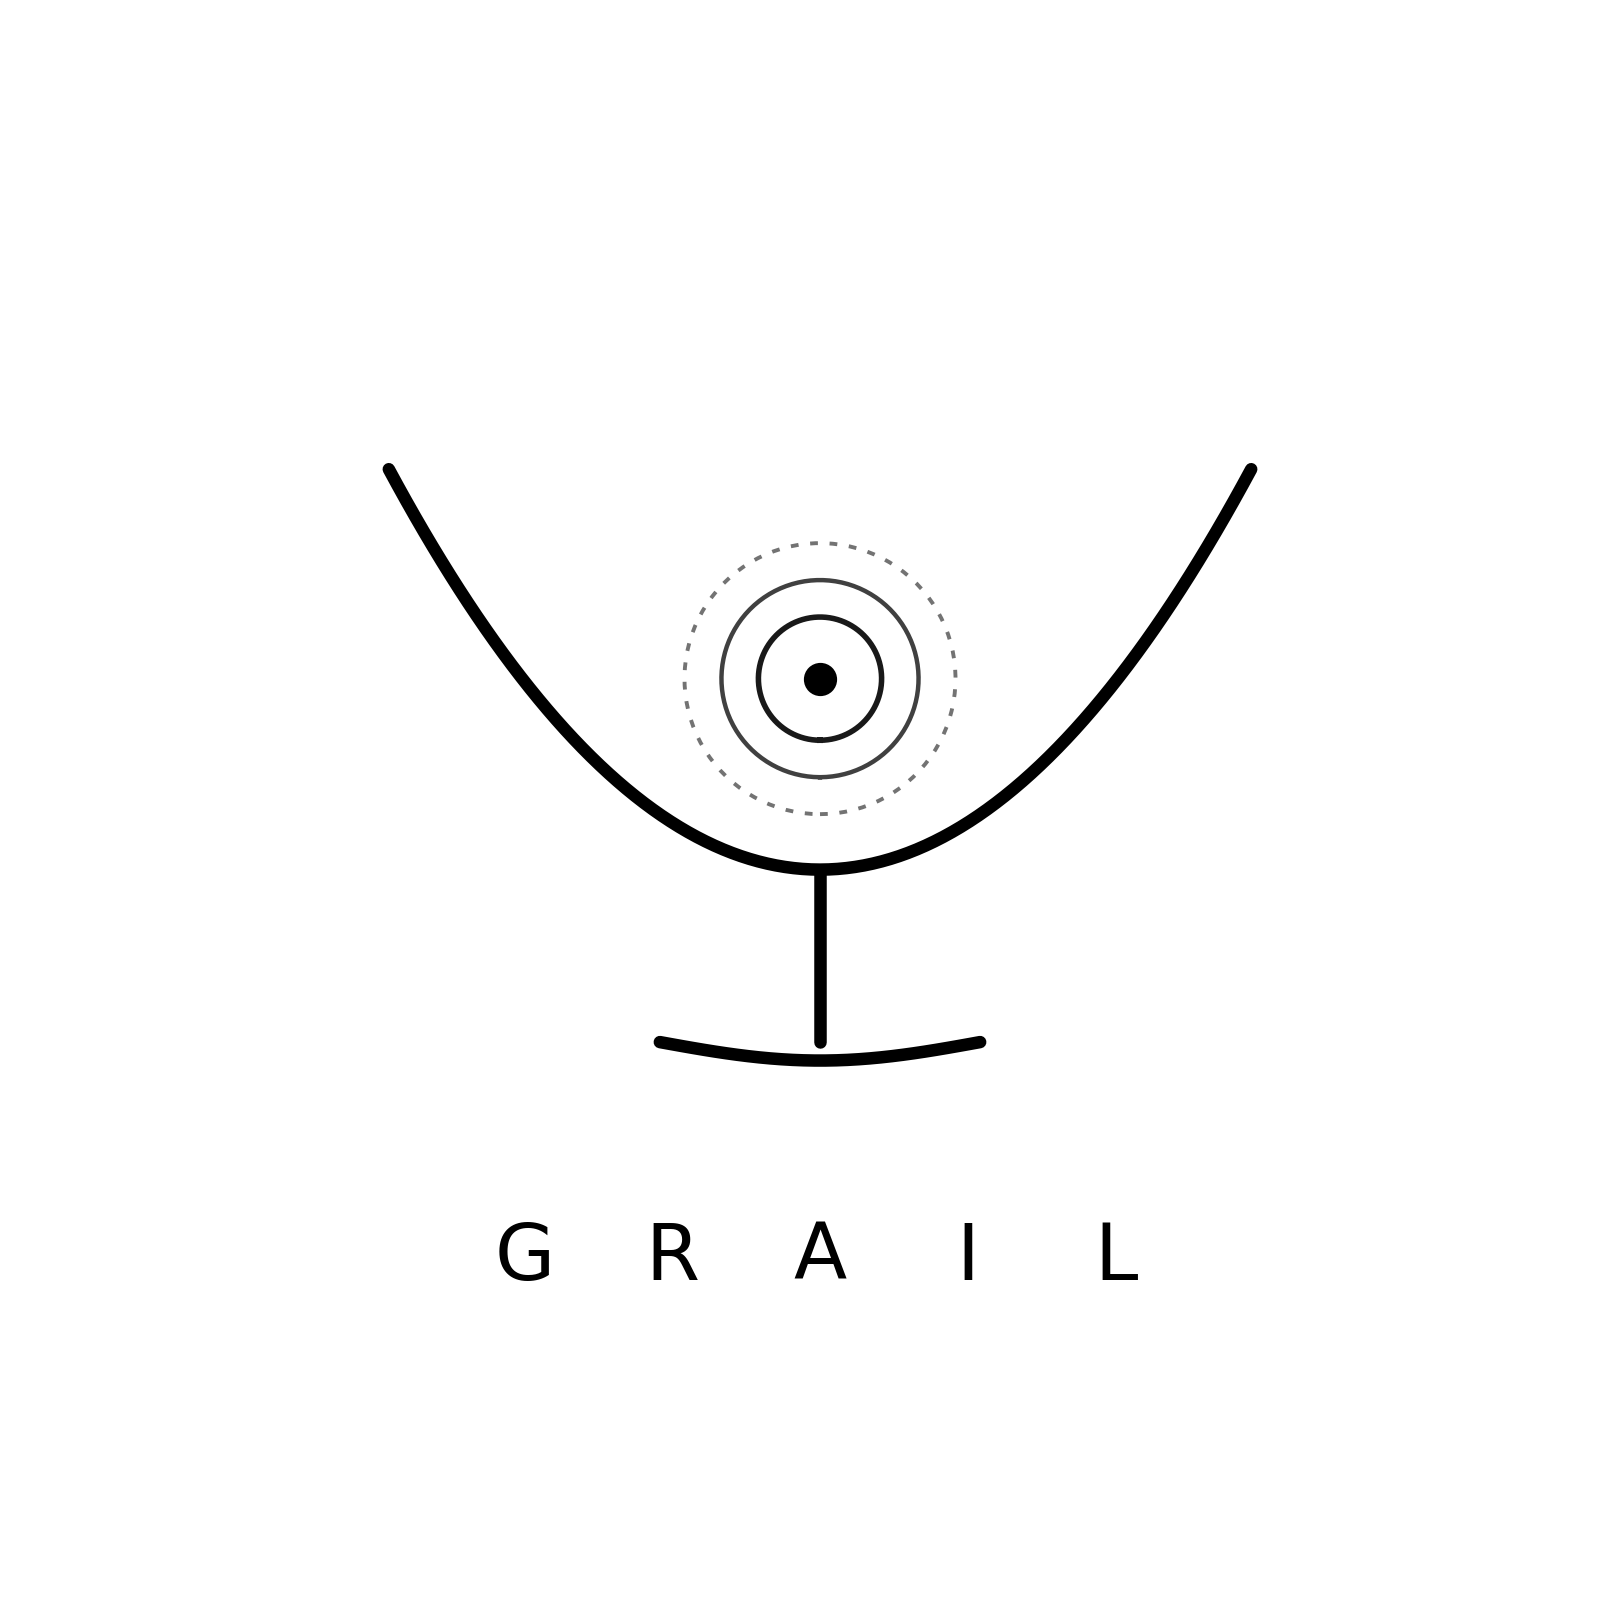
\includegraphics[width=0.54\textwidth,
      trim={350bp 280bp 300bp 420bp},clip]
      {../../logo/grail_logo_black_on_white_final.png}\par
    \vspace{0.35in}
    {\sffamily\bfseries\fontsize{30}{36}\selectfont\@title\par}
    \vspace{0.22in}
    {\large Green's-function Resolvent for\\[3pt]
      AI-accelerated Iteration Libraries\par}
    \vspace{0.30in}
    \begin{minipage}{0.90\textwidth}
      \centering
      #1\par
    \end{minipage}\par
    \vfill
    {\large\@author\par}
    \vspace{0.35in}
    {\small\@date\par}
    \vspace*{0.15in}
  \end{titlepage}
  \restoregeometry
  \hypersetup{pageanchor=true}%
}
\makeatother


\begin{document}
\sloppy

\makegrailcover{%
  \large A Portable Framework for Calibrated Uncertainty
  Quantification of Nonlinear Emulators in Coupled Fixed-Point Iterations\par
  \vspace{0.18in}
  \normalsize Mathematical Foundations and a 1-D NLTE Reference Implementation}

\begin{abstract}
\noindent Many of the most expensive simulations in science and
engineering follow a single pattern: a host code iterates a nonlinear
coupled system to convergence, and one block of that iteration ---
opacity, microphysics, subgrid closure, equation of state --- dominates
the cost.  AI surrogates trained against the truth solver promise
orders-of-magnitude speedups when they replace that block.  Examples
include radiative transfer with atomic-physics emulators, multigroup
neutrino transport with learned closures or collision operators,
opacity-driven radiation hydrodynamics, implicit hydrodynamics with
equation-of-state lookups, and learned subgrid closures in climate or
reactor codes.  The price is a per-call residual against ground truth
at every encounter, and as the iteration runs that residual is
re-injected at every cycle.  The converged-output error a user
actually sees is the sum over all those encounters, not the per-call
accuracy a held-out test set would report.

The structure is exactly multiple scattering --- the problem
classical and quantum scattering theory have solved for nearly a
century through the Lippmann--Schwinger equation.  A wave propagating
through an inhomogeneous medium scatters off the disturbance
repeatedly; the Lippmann--Schwinger equation closes the infinite
Born series of single, double, and $N$-fold scattering events into a
single resolvent acting on the disturbance.  An emulator-coupled
iteration meets the same residual at every cycle.  Replace the wave
by the converged simulation state, the scattering potential by the
per-call emulator residual, and the free propagator by the linearized
cycle's Green's function, and the Lippmann--Schwinger identity
transfers term for term: the converged-output error is the
discrete-iteration Born series, summed to all orders by the resolvent
$(\mathbf{I} - D\mathcal{T})^{-1}$.  GRAIL is that resolvent.  It is
evaluated matrix-free via GMRES on the composed host and emulator
Jacobian--vector products: the emulator contributes its JVP through
automatic differentiation; the host contributes its own through an
opaque callback.  GRAIL itself never imports either side, so the same
library wraps any simulation matching the pattern, and the calibrated
converged-output error band it produces has its coverage verified
split-conformally.

We make the abstraction concrete on three application testbeds drawn
from disjoint scientific communities: a one-dimensional plane-parallel
non-LTE atmosphere (two-level and five-level Balmer-H multilevel
configurations) --- the simplest physical setting that exercises every
component of the pipeline end to end against analytic anchors; the
self-consistent-field (SCF) electronic structure of stretched H$_2$
at the Coulson--Fischer triplet-instability point, with a neural
exchange--correlation surrogate; and a single-column
radiative--convective-equilibrium (RCE) climate column with a prescribed
affine heating law held fixed across numerical timesteps.  The same resolvent governs surrogate-error amplification
in all three.  The chapters that follow develop the wave-scattering
analogy in full (classical Helmholtz/Lippmann--Schwinger leading,
quantum scattering as specialization), derive the resolvent equation
from the elementary fixed-point statement and the implicit function
theorem, identify it as the $\Lambda$-iteration scattering Green's
function in the NLTE case, and cover the radiative-transfer
formulation and its analytic limits, the discretization, formal
solver, rate equations, ALI driver, four-tier test methodology, and
implementation status, with split-conformal calibration delivering a
distribution-free finite-sample coverage band on the converged
output under the stated exchangeability assumptions. Intermediate
derivations and integration contracts are written out explicitly.
\end{abstract}

\tableofcontents

% =============================================================================
\section*{Notation and Glossary}
\addcontentsline{toc}{section}{Notation and Glossary}
\label{sec:glossary}
% =============================================================================

This section collects every symbol used in the document, grouped by
role.  Symbols overloaded by context (the temperature $T$ versus the
cycle map $T$; the dimensionless frequency offset $x$ versus the state
vector $\mathbf{x}$) are listed under each meaning with a disambiguating
note.

\subsection*{Cycle, fixed point, and resolvent}

\noindent\begin{tabular}{@{}p{1.4in}p{4.8in}@{}}
\toprule
\textbf{Symbol} & \textbf{Meaning} \\ \midrule
$T(\mathbf{x})$ \emph{(map)} & Generic continuously differentiable cycle map $\mathbb{R}^n \to \mathbb{R}^n$; one round of radiation step composed with statistical-equilibrium (SE) step.  \emph{Distinct from} the temperature $T$ (italic, scalar), used in atomic-physics expressions. \\
$T_t \equiv \Tcyc_{\text{truth}}$ & Reference cycle: SE step is the closed-form rate-equation solver, equation~\eqref{eq:n2-over-n1}. \\
$T_e \equiv \Tcyc_{\text{emul}}$ & Emulator cycle: SE step is the APNN; $T_e = T_t + \dT$. \\
$\Trt$ & Radiation step: populations $\to$ source function $\to$ formal solve $\to$ $\Jbar$. \\
$\Tse$ & Statistical-equilibrium step: $(\Jbar, T, n_e) \to (n_1, n_2)$. \\
$\dT(\mathbf{x})$ & Per-cycle emulator residual, $\dT = T_e - T_t$.  Sampled at validation atmospheres; fed to GRAIL as the perturbation to be propagated. \\
$DT, D\Tcyc$ & Jacobian operator of the cycle, evaluated at a base point; $D\Tcyc = D\Tse \cdot D\Trt$ by chain rule. \\
$\rho(A)$ & Spectral radius of operator $A$: $\max_i |\lambda_i|$. \\
$(\mathbf{I}-DT)^{-1}$ & Resolvent of the linearized cycle; the Green's function summing all orders of emulator feedback through the coupled iteration. \\
$\mathbf{x}$ \emph{(state vector)} & Populations $(n_1, n_2)$ stacked over depth.  Shape \code{(N\_tau, 2)} inside \code{atmosphere/}; flat blocked layout \code{(2 N\_tau,)} at the GRAIL seam.  \emph{Distinct from} the dimensionless frequency offset $x$ (scalar). \\
$\mathbf{x}^*$ & A fixed point: $\mathbf{x}^* = T(\mathbf{x}^*)$. \\
$\mathbf{x}_t^*$, $\mathbf{x}_e^*$ & Truth and emulator fixed points respectively. \\
$\delta\mathbf{x}^*$ & Converged emulator displacement $\mathbf{x}_e^* - \mathbf{x}_t^*$; the quantity GRAIL predicts. \\
$F(\mathbf{x}, s)$ & Continuously parameterized residual function for the implicit-function-theorem existence argument; $F = \mathbf{x} - T_t(\mathbf{x}) - s\,\dT(\mathbf{x})$. \\
$R_2(\mathbf{v})$ & Second-order Taylor remainder of $T_t$ around $\mathbf{x}_t^*$; bounded as $\|R_2(\mathbf{v})\| \leq \tfrac{1}{2} M_{T_t} \|\mathbf{v}\|^2$. \\
$M_{T_t}$ & Uniform bound on the operator norm of $D^2 T_t$ over the relevant neighborhood. \\
\bottomrule
\end{tabular}

\subsection*{Radiation field and source function}

\noindent\begin{tabular}{@{}p{1.4in}p{4.8in}@{}}
\toprule
\textbf{Symbol} & \textbf{Meaning} \\ \midrule
$I_\nu(z, \mu)$, $I(\tau, x, \mu)$ & Specific intensity at frequency $\nu$ (or dimensionless offset $x$), depth $z$ (or optical depth $\tau$), direction cosine $\mu$.  Energy per unit frequency per unit time per unit area per unit solid angle. \\
$I^+, I^-$ & Upgoing ($\mu > 0$, propagating toward smaller $\tau$) and downgoing ($\mu < 0$) intensity components. \\
$J_\nu(\tau)$, $J(\tau, x)$ & Mean intensity, $\tfrac{1}{2}\int_{-1}^{+1} I_\nu \, d\mu$. \\
$\Jbar(\tau)$ & Line-profile-weighted mean intensity, $\Jbar = \int \phi(\nu) J_\nu \, d\nu = \int \phi(x) J(\tau, x) \, dx$.  This is the radiation-field input the rate equations consume. \\
$S_\nu, S_\nu(\tau)$ & Source function in general, $S_\nu = \eta_\nu / \chi_\nu$. \\
$\Sl(\tau)$ & Line source function (CRD: independent of frequency across the line); $\Sl = (1-\epsilon) \Jbar + \epsilon B$. \\
$B_\nu(T), B$ & Planck function at temperature $T$, frequency $\nu$.  In CRD/two-level expressions, $B$ without subscript is $B_{\nu_0}(T)$ at line center. \\
$\eta_\nu$ & Emissivity (energy emitted per unit volume per unit frequency per unit time per unit solid angle). \\
$\chi_\nu, \chi_l(\nu), \chi_l(\nu_0)$ & Total extinction coefficient (general / line / line-center). \\
\bottomrule
\end{tabular}

\subsection*{Line physics, atomic constants, and rates}

\noindent\begin{tabular}{@{}p{1.4in}p{4.8in}@{}}
\toprule
\textbf{Symbol} & \textbf{Meaning} \\ \midrule
$\epsilon$ & Photon destruction probability: $\epsilon \equiv C_\mathrm{ul}/(C_\mathrm{ul}+A_\mathrm{ul}\,\bar{B}(T))$, with $C_\mathrm{ul}$ the collisional de-excitation rate, $A_\mathrm{ul}$ the Einstein-A coefficient, and $\bar{B}(T)$ the angle-averaged stimulated-emission factor; $\epsilon \in (0, 1]$.  Pure scattering at $\epsilon \to 0$, pure LTE at $\epsilon = 1$. \\
$\phi_\nu, \phi(x)$ & Normalized line profile, $\int \phi_\nu \, d\nu = 1$.  In dimensionless form, $\phi(x) = e^{-x^2}/\sqrt{\pi}$ (Doppler). \\
$\psi(x)$ & Normalized absorption profile relative to line center, $\psi(x) = \phi_\nu/\phi_{\nu_0} = e^{-x^2}$. \\
$A_{21}$ & Einstein spontaneous-emission coefficient (s$^{-1}$). \\
$B_{12}, B_{21}$ & Einstein absorption / induced-emission coefficients.  Detailed balance: $g_1 B_{12} = g_2 B_{21}$, $A_{21} = (2 h\nu_0^3 / c^2) B_{21}$. \\
$C_{12}, C_{21}$ & Collisional excitation / de-excitation rates (s$^{-1}$).  Detailed-balance closure: $C_{12} = (g_2/g_1) e^{-h\nu_0/kT} C_{21}$. \\
$R_{12}, R_{21}$ & Total radiative transition rates (CRD-averaged): $R_{12} = B_{12} \Jbar$, $R_{21} = A_{21} + B_{21} \Jbar$. \\
$g_1, g_2$ & Statistical weights of the lower / upper level. \\
$n_1, n_2$ & Populations of the lower and upper levels (cm$^{-3}$). \\
$n_e$ & Free-electron number density (cm$^{-3}$). \\
$n_{\text{tot}}$ & Total population, $n_1 + n_2$. \\
$T$ \emph{(temperature, scalar)} & Local kinetic temperature.  \emph{Distinct from} the cycle map $T$ above (operator). \\
\bottomrule
\end{tabular}

\subsection*{Geometry and grids}

\noindent\begin{tabular}{@{}p{1.4in}p{4.8in}@{}}
\toprule
\textbf{Symbol} & \textbf{Meaning} \\ \midrule
$z$ & Physical height in plane-parallel atmosphere (cm). \\
$\tau$ & Line-center optical depth, $\tau = \int_z^\infty \chi_l(\nu_0)\, dz'$.  Grows inward. \\
$\tau_\nu$ & Frequency-dependent optical depth, $\tau_\nu = \psi(x)\,\tau$ for the static, single-line, fixed-broadening prototype. \\
$\tau_{\min}, \tau_{\max}$ & Depth grid bounds.  Defaults: $\tau_{\min} = 10^{-4}$, $\tau_{\max} \in \{10^2, 10^4, 10^6\}$. \\
$\nu, \nu_0$ & Frequency, line-center frequency. \\
$x$ \emph{(frequency offset)} & Dimensionless offset $x = (\nu - \nu_0)/\Delta\nu_D$.  \emph{Distinct from} the state vector $\mathbf{x}$ above (vector). \\
$\Delta\nu_D$ & Doppler width, $\Delta\nu_D = (\nu_0/c)\sqrt{2 k T_{\text{ref}}/m}$ at the relevant kinetic temperature $T_{\text{ref}}$. \\
$\mu$ & $\cos\theta$, where $\theta$ is the angle from outward normal.  Stored on $[0, 1]$ via reflection symmetry; sign determines up/down direction. \\
$N_\tau, N_\nu, N_\mu$ & Grid sizes.  Defaults: $N_\tau = 80$ (range $[40, 200]$), $N_\nu = 21$ (range $[11, 41]$), $N_\mu = 5$ (range $[3, 8]$). \\
$w_i$ \emph{(integration weights)} & Trapezoidal weights on the frequency grid, or Gauss--Legendre weights on the $\mu$ grid; context determines which. \\
$\xi_i, w_{\xi,i}$ & Gauss--Legendre nodes and weights on $[-1, 1]$, transformed to $[0, 1]$ via $\mu_i = (\xi_i+1)/2$, $w_i = w_{\xi,i}/2$. \\
\bottomrule
\end{tabular}

\subsection*{Lambda operator, ALI, and short characteristics}

\noindent\begin{tabular}{@{}p{1.4in}p{4.8in}@{}}
\toprule
\textbf{Symbol} & \textbf{Meaning} \\ \midrule
$\Lop$ & Linear integral operator mapping line source function to profile-weighted mean intensity, $\Jbar = \Lop \Sl$. \\
$\Lstar$ & Approximate Lambda operator used in ALI splitting, $\Lop = \Lstar + (\Lop - \Lstar)$.  In this work, $\Lstar = \mathrm{diag}(\Lop)$ (\citealt{OlsonAuerBuchler1986}). \\
$K_1(t)$ & Kernel of $\Lop$ in plane-parallel CRD with isotropic phase function, $K_1(t) = \tfrac{1}{2}\int \phi^2(x) E_1[\psi(x) t]\, dx$. \\
$E_1(z)$ & First exponential integral, $E_1(z) = \int_1^\infty t^{-1} e^{-z t}\, dt$. \\
$u$ & Dimensionless optical-depth increment along a single short-characteristic segment, $u = \psi(x)\,\Delta\tau / \mu$. \\
$\alpha(u), \beta(u)$ & Olson--Kunasz (1987) short-characteristics interpolation coefficients; $\alpha(u) = (1 - (1+u)e^{-u})/u$, $\beta(u) = (u - 1 + e^{-u})/u$. \\
\bottomrule
\end{tabular}

\subsection*{Universal physical constants}

\noindent\begin{tabular}{@{}p{1.4in}p{4.8in}@{}}
\toprule
\textbf{Symbol} & \textbf{Meaning} \\ \midrule
$h$ & Planck constant. \\
$k$ & Boltzmann constant. \\
$c$ & Speed of light. \\
\bottomrule
\end{tabular}

\subsection*{Code identifiers}

The following \code{typewriter}-font names refer to specific code
artifacts named in the technical reference and docs/testing.md:

{\small
\noindent\begin{tabular}{@{}p{2.0in}p{4.3in}@{}}
\toprule
\textbf{Identifier} & \textbf{Role} \\ \midrule
\code{atmosphere.grid}            & Depth, frequency, and angle-quadrature dataclasses. \\
\code{atmosphere.atmosphere}      & Atmosphere dataclass; isothermal and power-law constructors. \\
\code{atmosphere.formal\_solver}  & Short-characteristic formal solver (linear or parabolic OK87) and line-profile averaging. \\
\code{atmosphere.rate\_equations} & Closed-form two-level SE solve in master-$\epsilon$ form. \\
\code{atmosphere.fixed\_point}    & ALI driver (direct or iterative mode); cycle\_truth, cycle\_emulator. \\
\code{emulator.apnn}              & APNN model class (feed-forward, $\sim$34k params, softmax output). \\
\code{emulator.training}          & LHS data generator, training loop, validation split. \\
\code{emulator.jvp}               & Autograd JVP wrapper and cycle adapter. \\
\code{grail.api}                  & Public entry: resolvent\_solve, ResolventResult. \\
\code{grail.gmres}                & Matrix-free GMRES(m) with Arnoldi diagnostics. \\
\code{grail.jacobian}             & Composed JVP via chain rule; ($\mathbf{I} - D\Tcyc$) matvec. \\
\code{grail.pca}                  & SVD basis on validation residuals; per-PC propagation. \\
\code{grail.conformal}            & Split-conformal calibrator in observable space. \\
\code{decisions.runner}           & Amplification, GMRES and local-response checks. \\
\bottomrule
\end{tabular}
}

% =============================================================================
\section{Introduction}
\subsection{Scientific Context}
\label{sec:scientific-context}
A surrogate residual changes the state returned by one solver block.
The changed state affects subsequent calls to the coupled blocks, so its
effect on the converged solution depends on the complete feedback cycle.
GRAIL estimates that response through a matrix-free cycle resolvent.
The approximation is local in the surrogate perturbation; repeated
linear feedback is retained to all orders.

\subsection{Reference Implementations}
\label{sec:1d-testbed}
The radiative-transfer example uses a plane-parallel two-level atom with
prescribed thermodynamics, complete redistribution, and conserving
populations. The host transports radiation; a surrogate replaces the
statistical-equilibrium block. Analytic surface laws, population balance,
and independently solved linear systems provide verification targets.
Additional integrations exercise electronic structure and a climate column.
The shared radiative-transfer library retains the three-level analytic
host checks and the five-level hybrid population model.
The climate example uses a prescribed affine heating law and varies
the numerical timestep at fixed physical heating, rather than varying
a physical climate-feedback parameter.

\subsection{Using This Guide}
\label{sec:document-roadmap}
Section~\ref{sec:methodology} develops the response mathematics.
Sections~\ref{sec:rt-problem} and \ref{sec:scf-testbed} explain the
reference physics. Sections~\ref{sec:resolvent}--\ref{sec:fixed-point}
specify callbacks, coordinates, discretization, and solver contracts.
Section~\ref{sec:tests} describes verification, and the companion
user manual gives installation and runnable integration recipes.

\section{Methodology}
\label{sec:methodology}

\subsection{Motivation: Wave Scattering}
\label{sec:lippmann-schwinger}

The structural problem GRAIL solves is the discrete-iteration analog
of one of the oldest problems in mathematical physics: summing a small
perturbation through all orders of multiple scattering.

\paragraph{Why scattering is the right analogy.}
Wave scattering is not just one example of a self-consistent equation.
It is the prototype of a particular physical situation that recurs
throughout mathematical physics, and that emulator-coupled iteration
realizes exactly.  The situation has three ingredients.  First, a
known, already-solved unperturbed system: in scattering, a free wave
running through a uniform background; in GRAIL, the converged truth
simulation.  Second, a small localized disturbance that the system
must respond to but cannot handle in closed form: in scattering, a
patch of inhomogeneous medium (or, in the quantum case, a localized
potential); in GRAIL, the per-call residual left behind when the
truth solver is replaced by a learned surrogate.  Third---and this is
the part that ties the analogy together---the perturbation acts on
the system not once but through \emph{repeated encounters as the
system propagates through its own state space}.  A wave in the
scattering region bounces off the inhomogeneity many times before it
escapes; a coupled-iteration simulation revisits its emulated block
on every cycle, and each visit injects another copy of the residual
into the iteration that follows.  In both problems the converged
response is not the single-encounter response.  It is the sum over
\emph{all} encounter histories, ordered by encounter count, with the
unperturbed propagator carrying the system between successive
encounters with the same fixed perturbation.  This is exactly what
the Born series writes down.  We derive it below first for classical
waves and then for quantum particles, and we transfer it to GRAIL
term for term in \S\ref{sec:resolvent-greens-function}.  Once we see
that emulator-coupled iteration is a multiple-scattering problem---the
system meets the same residual on every cycle---every tool classical
scattering theory has built (Born expansion, distorted-wave
preconditioning, multiple-scattering convergence criteria) is
available, off the shelf, for emulator uncertainty quantification.

The cleanest formal setting for this multiple-scattering structure is
a classical wave propagating through an inhomogeneous medium,
described by the Helmholtz equation with a contrast term and its
Lippmann--Schwinger integral form \citep{LippmannSchwinger1950}.  We
sketch the derivation here for classical waves, specialize it to the
quantum-mechanical case, and then show in the rest of the section
that emulator-coupled iteration produces a structurally identical
equation.  Every conceptual ingredient of GRAIL---the resolvent, the
Green's function, the Born series, the diagonal preconditioner, the
second-order error term---has a direct counterpart in the scattering
theory below.  The convergence and preconditioning machinery that
scattering theory has built up over eight decades carries over to
GRAIL directly.

\subsubsection{Classical waves: Helmholtz and Lippmann--Schwinger}

The Lippmann--Schwinger equation is not really a quantum equation.
It is the equation any wave obeys when it propagates through an
inhomogeneous medium, and we can write it down without any reference
to quantum mechanics at all.  Consider a scalar field
$\psi(\mathbf{r})$ at fixed wavenumber $k$ obeying the inhomogeneous
Helmholtz equation
\begin{equation}
(\nabla^2 + k^2)\,\psi(\mathbf{r}) \;=\; V(\mathbf{r})\,\psi(\mathbf{r}),
\label{eq:helmholtz-V}
\end{equation}
where $V(\mathbf{r})$ is the disturbance---the contrast between the
medium and its uniform background, multiplied by whatever physical
prefactor turns the wave equation in the medium into the wave
equation in the background plus a source (sign convention chosen so
the Lippmann--Schwinger equation below carries the standard $+\,G_0 V$
form).  For a sound wave in a
fluid of density $\rho_0 + \delta\rho(\mathbf{r})$, $V$ is built from
$\delta\rho/\rho_0$.  For a light wave passing through a region with
refractive index $n_0 + \delta n(\mathbf{r})$, $V$ is built from
$\delta n / n_0$.  For a seismic wave through a heterogeneity in the
Earth, $V$ is built from the local contrast in elastic moduli.  In
every case~\eqref{eq:helmholtz-V} is the same mathematical object.

The free-space Green's function $G_0(\mathbf{r}, \mathbf{r}')$ obeys
\begin{equation}
(\nabla^2 + k^2)\, G_0(\mathbf{r}, \mathbf{r}')
\;=\; \delta(\mathbf{r} - \mathbf{r}'),
\label{eq:helmholtz-greens}
\end{equation}
and in three dimensions it has the familiar outgoing-wave form
$G_0(\mathbf{r}, \mathbf{r}') = -\,e^{ik|\mathbf{r}-\mathbf{r}'|} /
(4\pi |\mathbf{r}-\mathbf{r}'|)$.  Two facts now combine to give the
closed integral form.  First, the unperturbed medium itself is a
free-wave background: any solution $\psi_0$ of the homogeneous
equation $(\nabla^2 + k^2)\,\psi_0 = 0$---an incident plane wave, for
instance---is a self-consistent state in the absence of the
disturbance.  Second, $G_0$ inverts the Helmholtz operator on
sources: for any function $f(\mathbf{r}')$, the convolution
$\int G_0(\mathbf{r}, \mathbf{r}')\,f(\mathbf{r}')\,d^3\!r'$
satisfies, by direct application of \eqref{eq:helmholtz-greens},
\begin{equation}
(\nabla^2 + k^2)\,\!\left[\int G_0(\mathbf{r}, \mathbf{r}')\,
f(\mathbf{r}')\,d^3\!r'\right]
\;=\; \int \delta(\mathbf{r} - \mathbf{r}')\,f(\mathbf{r}')\,d^3\!r'
\;=\; f(\mathbf{r}).
\end{equation}

Decompose the full field as $\psi = \psi_0 + \delta\psi$ and substitute
into \eqref{eq:helmholtz-V}; since $\psi_0$ is annihilated by
$(\nabla^2 + k^2)$, we are left with
\begin{equation}
(\nabla^2 + k^2)\,\delta\psi(\mathbf{r}) \;=\; V(\mathbf{r})\,\psi(\mathbf{r}),
\label{eq:helmholtz-deltapsi}
\end{equation}
where the right-hand side carries the \emph{full} $\psi$, not just
$\psi_0$---this is the self-consistency that turns the equation into a
fixed-point statement rather than a one-step solve.  Inverting
$(\nabla^2 + k^2)$ via $G_0$ gives
\begin{equation}
\delta\psi(\mathbf{r}) \;=\; \int G_0(\mathbf{r}, \mathbf{r}')\,
V(\mathbf{r}')\,\psi(\mathbf{r}')\,d^3\!r' .
\label{eq:deltapsi-integral}
\end{equation}
Adding back the unperturbed wave $\psi_0$ yields the classical-wave
Lippmann--Schwinger equation,
\begin{equation}
\boxed{\;\psi(\mathbf{r}) \;=\; \psi_0(\mathbf{r}) +
\int G_0(\mathbf{r}, \mathbf{r}')\,V(\mathbf{r}')\,\psi(\mathbf{r}')\,
d^3\!r' .\;}
\label{eq:LS-classical}
\end{equation}
This is a self-consistent integral relation in $\psi$: the field at
any point is the field that would have been there in the absence of
the disturbance, plus a correction built by integrating the
disturbance against the free-space Green's function.  Iterating
\eqref{eq:LS-classical} by repeated substitution generates the Born
series in $G_0 V$.  The procedure is mechanical: substitute the
right-hand side of \eqref{eq:LS-classical} for the $\psi$ that appears
inside the integral, then for the $\psi$ that appears in the resulting
double integral, and so on.  The first substitution gives
\begin{multline}
\psi(\mathbf{r}) \;=\; \psi_0(\mathbf{r})
  + \int G_0(\mathbf{r}, \mathbf{r}_1)\,V(\mathbf{r}_1)\,\psi_0(\mathbf{r}_1)\,d^3\!r_1 \\
  + \iint G_0(\mathbf{r}, \mathbf{r}_1)\,V(\mathbf{r}_1)\,
          G_0(\mathbf{r}_1, \mathbf{r}_2)\,V(\mathbf{r}_2)\,\psi(\mathbf{r}_2)\,
          d^3\!r_1\,d^3\!r_2 ,
\end{multline}
already showing the structure: each insertion of $V$ scatters the wave
locally, and a free propagator $G_0$ carries it from the previous
scattering site to the next.  Continuing the substitution to all
orders produces
\begin{equation}
\psi(\mathbf{r}) \;=\; \psi_0(\mathbf{r}) +
\sum_{k=1}^{\infty}\,
\idotsint
G_0(\mathbf{r}, \mathbf{r}_1)\,V(\mathbf{r}_1)\,
G_0(\mathbf{r}_1, \mathbf{r}_2)\,V(\mathbf{r}_2)\cdots
G_0(\mathbf{r}_{k-1}, \mathbf{r}_k)\,V(\mathbf{r}_k)\,\psi_0(\mathbf{r}_k)\,
d^3\!r_1\cdots d^3\!r_k .
\label{eq:born-classical-explicit}
\end{equation}
The $k$-th term is the wave scattered exactly $k$ times by $V$, at
successive locations $\mathbf{r}_1, \mathbf{r}_2, \ldots, \mathbf{r}_k$,
with $G_0$ propagating it freely between scatterings, before it is
observed at $\mathbf{r}$.  The structure is transparent in operator
notation.  We now reinterpret the same symbols as linear operators
on wavefunctions: $V$ is multiplication by the function
$V(\mathbf{r})$, and $G_0$ is convolution against the kernel
$G_0(\mathbf{r}, \mathbf{r}')$ (the inverse of $\nabla^2 + k^2$).  In
that reading the composite $G_0 V$ is the
``scatter-once-then-propagate'' operator, $(G_0 V)^k$ is its $k$-fold
composition (which when written out is exactly the $k$-fold integral
kernel of eqn~\eqref{eq:born-classical-explicit}), and the series
collapses to a geometric one in $G_0 V$,
\begin{equation}
\psi \;=\; \psi_0 + (G_0 V)\,\psi_0 + (G_0 V)^2\,\psi_0 + (G_0 V)^3\,\psi_0 + \cdots
\;=\; (\mathbf{I} - G_0 V)^{-1}\,\psi_0 ,
\label{eq:born-classical-operator}
\end{equation}
provided the spectral radius $\rho(G_0 V) < 1$, the convergence
condition for the geometric series.  The closed form on the
right-hand side of \eqref{eq:born-classical-operator} is the
free-space Green's function $G_0$ \emph{dressed} by all orders of
multiple scattering off the disturbance $V$.  The same identity
appears, with the same structure and the same convergence condition,
in the quantum-mechanical setting (\S\ref{sec:quantum-scattering});
only the physical interpretation of the wave $\psi$ and the disturbance
$V$ changes.  The Mattuck-style Feynman-diagram reading of the same
series, with each $V$ a vertex and each $G_0$ an arrow, is
Figure~\ref{fig:born-series}.

\subsubsection{Quantum scattering: the same equation, and its GRAIL counterpart}
\label{sec:quantum-scattering}

The classical Lippmann--Schwinger
equation~\eqref{eq:LS-classical} first appeared, in essentially
identical form, in quantum-mechanical scattering theory, where it
takes its canonical name.  Consider a particle of energy $E$
scattering off a localized potential $V$, with the background
described by the free Hamiltonian $H_0$.  The full Hamiltonian is
$H = H_0 + V$, and the time-independent Schr\"odinger equation is
\begin{equation}
(E - H_0 - V)\,\psi = 0 .
\label{eq:schrodinger}
\end{equation}
We would like to solve this for $\psi$ by moving $V\psi$ to the
right-hand side and dividing through by $(E - H_0)$:
\begin{equation}
(E - H_0)\,\psi \;=\; V\,\psi .
\label{eq:schrodinger-rearranged}
\end{equation}
The trouble is that $(E - H_0)$ has zero eigenvalues: the
free-particle eigenstates $\psi_0$ at the same energy $E$ obey
$(E - H_0)\,\psi_0 = 0$ by definition, so the operator has no
ordinary inverse.  Formally we would like to write $\psi = (E -
H_0)^{-1}\,V\,\psi$, but the inverse fails to exist on the energy
shell.  The standard remedy is to add a small imaginary part
$i\epsilon$ to $E$, which displaces the singularity off the real
axis and selects outgoing-wave boundary conditions in the limit
$\epsilon \to 0^+$.  The result is the \emph{free-particle Green's
function}, or \emph{free propagator},
\begin{equation}
G_0(E) \;\equiv\; (E - H_0)^{-1},
\label{eq:G0}
\end{equation}
the linear operator that takes a source in the unperturbed problem
to the system's response.  In the operator-theoretic and
mathematical-physics literature the same object is called the
\emph{resolvent} of $H_0$ at energy $E$, a name that emphasizes its
analytic structure as a function of complex $E$ --- with poles at
the bound-state eigenvalues and a branch cut along the continuous
spectrum.  We use both names interchangeably.  In three dimensions
at energy $E = \hbar^2 k^2 / 2m$, $G_0$ has the familiar
outgoing-spherical-wave form $G_0(\mathbf{r}, \mathbf{r}')
\propto e^{ik|\mathbf{r}-\mathbf{r}'|}/|\mathbf{r}-\mathbf{r}'|$,
the same shape as the classical Helmholtz Green's function in
\S\ref{sec:lippmann-schwinger}.  Applying $G_0$ to both sides
of~\eqref{eq:schrodinger-rearranged} and adding the homogeneous
piece $\psi_0$, we get
\begin{equation}
\boxed{\;\psi = \psi_0 + G_0\,V\,\psi ,\;}
\label{eq:LS}
\end{equation}
the \emph{Lippmann--Schwinger equation}.  It is exact.  No
approximation has been made.

The shape of~\eqref{eq:LS} is the shape GRAIL inherits in the
discrete-iteration setting.  GRAIL replaces a single block of a
coupled-iteration simulation with a learned surrogate, and the
surrogate's per-call residual against the truth solver is the
discrete-iteration analog of the scattering potential $V$.  The truth
simulation already converges to its fixed point; this fixed point plays
the role of the unperturbed quantum state $\psi_0$.  The linearized
reference cycle has its own resolvent operator (derived rigorously in
\S\ref{sec:linearization} below), and that resolvent plays the role
of the free Green's function $G_0$.
With these identifications,
\begin{center}
\renewcommand{\arraystretch}{1.2}
\begin{tabular}{@{}lcl@{}}
\toprule
\textbf{quantum scattering} & $\quad\longleftrightarrow\quad$ & \textbf{GRAIL coupled iteration} \\ \midrule
incident wave $\psi_0$              &  & truth fixed point $\mathbf{x}_t^*$ \\
scattering potential $V$            &  & per-call emulator residual $\dT$ \\
free Green's function $G_0$         &  & cycle resolvent $(\mathbf{I} - DT_t)^{-1}$ \\
scattering correction $\psi - \psi_0$ &  & converged displacement $\delta\mathbf{x}^*$ \\
distorted-wave Born approx.\        &  & ALI diagonal-$\Lstar$ preconditioner \\
\bottomrule
\end{tabular}
\end{center}
the converged emulator-coupled state obeys an equation that is
structurally identical to~\eqref{eq:LS}: the GRAIL resolvent equation
\begin{equation}
\boxed{\;\delta\mathbf{x}^{*} = (\mathbf{I} - DT_t)^{-1}\,\dT(\mathbf{x}_e^*) + \mathcal{O}(\|\dT\|^2) ,\;}
\label{eq:resolvent-preview}
\end{equation}
in which $(\mathbf{I} - DT_t)^{-1}$ acts as a Green's function for the
cycle operator (\S\ref{sec:resolvent-greens-function}), $\dT$ acts as
the perturbing potential, and $\delta\mathbf{x}^*$ is the converged
response.  We derive~\eqref{eq:resolvent-preview} from first
principles in \S\ref{sec:linearization}.  Below we develop the analogy
further by showing that the scattering Born series and the GRAIL
iteration-amplification series are the same construction.

\subsubsection{The Born series and its physical interpretation}

Equation~\eqref{eq:LS} is implicit in $\psi$: the unknown quantum state
appears on both sides.  The standard resolution is to iterate, which
generates the \emph{Born series},
\begin{equation}
\psi = \psi_0 + G_0 V\,\psi_0 + G_0 V\,G_0 V\,\psi_0 + (G_0 V)^3 \psi_0 + \cdots ,
\label{eq:born-LS}
\end{equation}
which is equivalently the formal closed-form sum
\begin{equation}
\psi = (\mathbf{I} - G_0 V)^{-1}\,\psi_0
\label{eq:LS-resolvent}
\end{equation}
provided $\mathbf{I} - G_0 V$ is invertible (equivalently, the
spectral radius $\rho(G_0 V) < 1$, the convergence condition of the
geometric series).  Each term of~\eqref{eq:born-LS} has a transparent
physical reading.  $\psi_0$ is the incident wave; $G_0 V\,\psi_0$ is
the wave scattered once by $V$ and propagated to the observation
point; $(G_0 V)^k\,\psi_0$ is the wave scattered exactly $k$ times.
The geometric resummation in~\eqref{eq:LS-resolvent} is exact: all
orders of multiple scattering are summed, and the closed form is the
free Green's function $G_0$ ``dressed'' by the perturbation $V$.
Figure~\ref{fig:born-series} shows the algebraic series, the
corresponding multiple-scattering diagrams, and the equivalent
self-consistent (Dyson) form side by side.

\begin{figure}[ht]
\centering
\resizebox{\textwidth}{!}{%
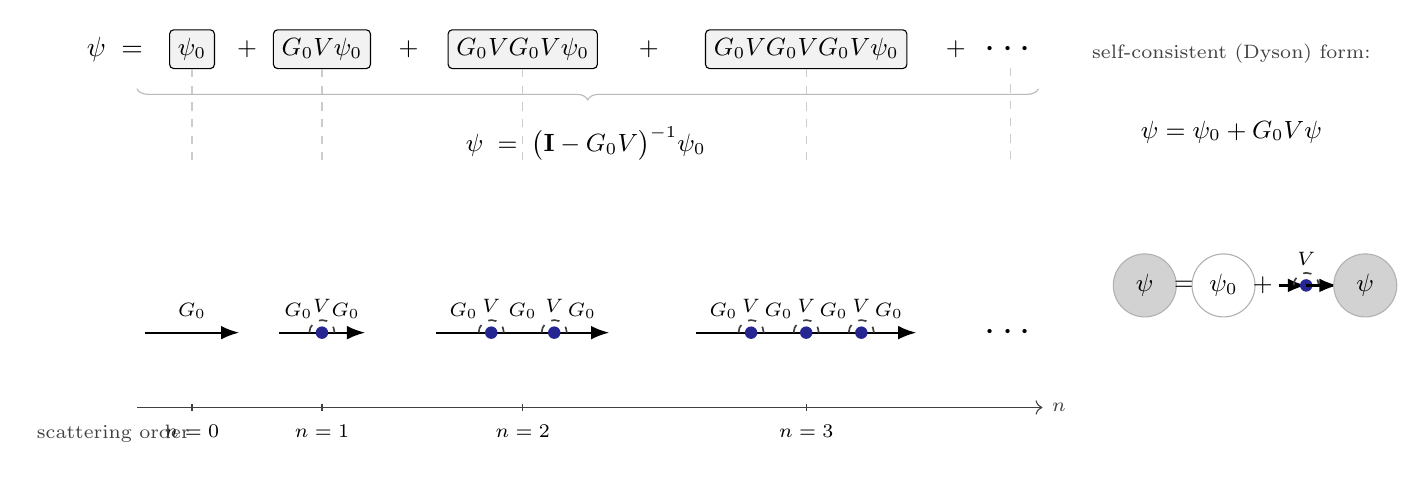
\begin{tikzpicture}[
  every node/.style={font=\small},
  algbox/.style={draw, rounded corners=1.5pt, fill=gray!10, inner sep=3pt, font=\small},
  vert/.style={circle, fill=blue!50!black!85, inner sep=0pt, minimum size=4.5pt},
  prop/.style={-Latex, thick, black},
  Vline/.style={dashed, semithick, gray!50!black},
  Vlabel/.style={font=\small, anchor=south, inner sep=1pt},
  guide/.style={dashed, gray!40, thin},
]
% --- Top row: algebraic Born series ---
\node[anchor=east, font=\normalsize] at (-0.2, 2.0) {$\psi \;=$};
\node[algbox] (a0) at (0.3, 2.0)  {$\psi_0$};
\node                              at (1.0, 2.0) {$+$};
\node[algbox] (a1) at (1.95, 2.0) {$G_0 V \psi_0$};
\node                              at (3.05, 2.0) {$+$};
\node[algbox] (a2) at (4.5, 2.0)  {$G_0 V G_0 V \psi_0$};
\node                              at (6.1, 2.0) {$+$};
\node[algbox] (a3) at (8.1, 2.0)  {$G_0 V G_0 V G_0 V \psi_0$};
\node                              at (10.0, 2.0) {$+$};
\node[font=\Large] (adots) at (10.7, 2.0) {$\cdots$};
% --- Closed-form resummation underneath the algebraic row ---
\draw[gray!55, decoration={brace, mirror, raise=1.5pt, amplitude=4pt}, decorate]
  (-0.4, 1.55) -- (11.05, 1.55);
\node at (5.3, 0.8) {$\psi \;=\; \bigl(\mathbf{I} - G_0 V\bigr)^{-1}\psi_0$};
% --- Bottom row: Feynman diagrams (Mattuck convention) ---
%  - solid arrow line     = free propagator G_0
%  - filled circle vertex = scattering point on the propagator
%  - semicircular arc     = one V insertion (Mattuck-style external
%                           interaction); each arc above the propagator
%                           represents one factor of V acting at the
%                           vertex below it.
\def\diagy{-1.6}     % propagator line height
\def\Varc{0.16}      % radius of the V semicircle
% n=0: bare propagator (no V insertions)
\draw[prop] (-0.3, \diagy) -- (0.9, \diagy);
\node[font=\scriptsize, anchor=south] at (0.3, \diagy+0.05) {$G_0$};
% n=1: single scattering
\draw[prop] (1.4, \diagy) -- (2.5, \diagy);
\node[vert] (v1) at (1.95, \diagy) {};
\draw[Vline] (1.95-\Varc, \diagy) arc[start angle=180, end angle=0, radius=\Varc];
\node[Vlabel, font=\scriptsize] at (1.95, \diagy+\Varc+0.05) {$V$};
\node[font=\scriptsize, anchor=south] at (1.65, \diagy+0.05) {$G_0$};
\node[font=\scriptsize, anchor=south] at (2.25, \diagy+0.05) {$G_0$};
% n=2: double scattering
\draw[prop] (3.4, \diagy) -- (5.6, \diagy);
\node[vert] (v2a) at (4.1, \diagy) {};
\node[vert] (v2b) at (4.9, \diagy) {};
\draw[Vline] (4.1-\Varc, \diagy) arc[start angle=180, end angle=0, radius=\Varc];
\node[Vlabel, font=\scriptsize] at (4.1, \diagy+\Varc+0.05) {$V$};
\draw[Vline] (4.9-\Varc, \diagy) arc[start angle=180, end angle=0, radius=\Varc];
\node[Vlabel, font=\scriptsize] at (4.9, \diagy+\Varc+0.05) {$V$};
\node[font=\scriptsize, anchor=south] at (3.75, \diagy+0.05) {$G_0$};
\node[font=\scriptsize, anchor=south] at (4.5, \diagy+0.05) {$G_0$};
\node[font=\scriptsize, anchor=south] at (5.25, \diagy+0.05) {$G_0$};
% n=3: triple scattering
\draw[prop] (6.7, \diagy) -- (9.5, \diagy);
\node[vert] (v3a) at (7.4, \diagy) {};
\node[vert] (v3b) at (8.1, \diagy) {};
\node[vert] (v3c) at (8.8, \diagy) {};
\draw[Vline] (7.4-\Varc, \diagy) arc[start angle=180, end angle=0, radius=\Varc];
\node[Vlabel, font=\scriptsize] at (7.4, \diagy+\Varc+0.05) {$V$};
\draw[Vline] (8.1-\Varc, \diagy) arc[start angle=180, end angle=0, radius=\Varc];
\node[Vlabel, font=\scriptsize] at (8.1, \diagy+\Varc+0.05) {$V$};
\draw[Vline] (8.8-\Varc, \diagy) arc[start angle=180, end angle=0, radius=\Varc];
\node[Vlabel, font=\scriptsize] at (8.8, \diagy+\Varc+0.05) {$V$};
\node[font=\scriptsize, anchor=south] at (7.05, \diagy+0.05) {$G_0$};
\node[font=\scriptsize, anchor=south] at (7.75, \diagy+0.05) {$G_0$};
\node[font=\scriptsize, anchor=south] at (8.45, \diagy+0.05) {$G_0$};
\node[font=\scriptsize, anchor=south] at (9.15, \diagy+0.05) {$G_0$};
% n=...:
\node[font=\Large] at (10.7, \diagy) {$\cdots$};
% --- Dashed vertical guides connecting algebraic terms to diagrams ---
\draw[guide] (a0.south)    -- (0.3, 0.5);
\draw[guide] (a1.south)    -- (1.95, 0.5);
\draw[guide] (a2.south)    -- (4.5, 0.5);
\draw[guide] (a3.south)    -- (8.1, 0.5);
\draw[guide] (adots.south) -- (10.7, 0.5);
% --- Scattering-order axis ---
\draw[->, thin, gray!50!black] (-0.4, -2.55) -- (11.1, -2.55);
\node[font=\scriptsize, gray!50!black, anchor=west] at (11.1, -2.55) {$n$};
\foreach \x/\n in {0.3/0, 1.95/1, 4.5/2, 8.1/3} {
  \draw[gray!50!black, thin] (\x, -2.50) -- (\x, -2.60);
  \node[font=\scriptsize, anchor=north] at (\x, -2.65) {$n=\n$};
}
\node[font=\scriptsize, gray!50!black, anchor=north] at (-0.7, -2.65)
  {scattering order};
% --- Dyson self-consistent inset (right) ---
%   blob = G_0 + G_0 -> V (cross) -> blob
\node[font=\scriptsize, anchor=south, gray!50!black] at (13.5, 1.7)
  {self-consistent (Dyson) form:};
\node[anchor=center] at (13.5, 0.95)
  {$\psi = \psi_0 + G_0 V \psi$};
\node[fill=gray!35, draw=gray!60, circle, minimum size=8mm] (blob1) at (12.4, -1.0) {$\psi$};
\node                              at (12.9, -1.0) {$=$};
\node[fill=white, draw=gray!60, circle, minimum size=8mm] (psi0) at (13.4, -1.0) {$\psi_0$};
\node                              at (13.9, -1.0) {$+$};
\draw[prop] (14.1, -1.0) -- (14.45, -1.0);
\node[vert] (vd) at (14.45, -1.0) {};
\draw[Vline] (14.45-\Varc, -1.0) arc[start angle=180, end angle=0, radius=\Varc];
\node[Vlabel, font=\scriptsize] at (14.45, -1.0+\Varc+0.05) {$V$};
\draw[prop] (14.45, -1.0) -- (14.85, -1.0);
\node[fill=gray!35, draw=gray!60, circle, minimum size=8mm] (blob2) at (15.2, -1.0) {$\psi$};
\end{tikzpicture}%
}
\caption{Born series of the Lippmann--Schwinger
equation~\eqref{eq:LS}, drawn in the Feynman-diagram convention of
\citet[Ch.~3]{Mattuck1992} for single-particle scattering off an
external potential.  Top row: the algebraic Neumann expansion
$\psi = \psi_0 + G_0 V\,\psi_0 + (G_0 V)^2\,\psi_0 + \cdots$, each term
in its own light-gray rounded box.  Bottom row: the corresponding
Feynman diagrams---a solid horizontal arrow for the free propagator
$G_0$, filled circles for scattering vertices on the propagator line,
and a semicircular arc above each vertex (Mattuck's convention)
denoting one insertion of the perturbing potential $V$.  Each power
of $G_0 V$ corresponds to one additional scattering event off $V$,
propagated by $G_0$ between events; the geometric resummation
collapses the infinite expansion into the resolvent
$\bigl(\mathbf{I} - G_0 V\bigr)^{-1}$.  Right-hand inset: the
equivalent self-consistent (Dyson) form $\psi = \psi_0 + G_0 V \psi$,
with an open circle for the unperturbed state $\psi_0$ and a shaded
blob for the dressed state $\psi$ on both sides of the
equation---the graphical statement that the infinite expansion and
the operator inversion are the same object.  In the GRAIL setting
(\S\ref{sec:resolvent-greens-function}), the same diagrams describe
the iteration-amplification series with
$G_0 \mapsto (\mathbf{I} - DT_t)^{-1}$, $V \mapsto \dT$, and the
dressed state $\mapsto \delta\mathbf{x}^{*}$.}
\label{fig:born-series}
\end{figure}

GRAIL inherits this structure term for term.  Iterating the
discrete-iteration analog~\eqref{eq:resolvent-preview} produces the
GRAIL Born series,
\begin{equation}
\delta\mathbf{x}^{*} = \dT + DT_t\,\dT + (DT_t)^2\,\dT + (DT_t)^3\,\dT + \cdots ,
\label{eq:born-grail}
\end{equation}
in which the leading term $\dT$ is the bare per-call emulator
residual---what one-shot, in-distribution validation measures---and
term $k$ is the residual after exactly $k$ further round-trips
through the host cycle.  This is the iteration-amplification effect
that motivates the present work: the part of the converged-output
error that standalone validation cannot see.  Where scattering theory
sums multiple scattering of an incident wave by the potential $V$,
GRAIL sums multiple feedback of the per-call emulator residual through
the host cycle.  The closed-form resummation~\eqref{eq:resolvent-preview}
is the discrete-iteration counterpart of~\eqref{eq:LS-resolvent}.
GRAIL evaluates this closed form implicitly through GMRES on
$(\mathbf{I} - D\Tcyc)$, which is matrix-free in $D\Tcyc$, so we never
build the geometric sum term by term.

A subtle point worth pausing on.  The GRAIL Born
series~\eqref{eq:born-grail} is linear in the emulator residual $\dT$,
but it is \emph{all orders} in the cycle Jacobian $D\Tcyc$.  Truncating
after the first two terms --- the Neumann expansion stopped at
$\dT + D\Tcyc\,\dT$ --- looks tempting because each term is linear in
$\dT$, but it misses precisely the regime where GRAIL is interesting.
At a cycle spectral radius $\rho(D\Tcyc) = 0.99$, the two-term
truncation gives $1.99\,\dT$ while the full geometric sum gives
$100\,\dT$ (the resolvent ratio $1/(1-\rho)$).  Each additional term is
only a factor $\rho$ smaller than the previous, so the high-order
terms pile up rather than vanish.  The amplification GRAIL is built
to capture lives in those high-order terms, and the matrix-free GMRES
on $(\mathbf{I} - D\Tcyc)$ is what sums them all in one linear-system
call.

The classical and quantum derivations above share a single underlying
equation.  Whether the wave is a probability amplitude, a sound
pressure, an electromagnetic mode, a seismic stress wave, or---as we
will see in \S\ref{sec:resolvent-greens-function}---a converged
displacement in a coupled iteration, the operator algebra collapses
to the same resolvent identity
\begin{equation}
G \;=\; G_0 + G_0\,V\,G,
\label{eq:resolvent-identity}
\end{equation}
and the identity does not know what the thing propagating is.  Within
radiative transfer itself the same identity reappears: the converged
line source function $S_l^*$ obeys
$(\mathbf{I} - (1 - \epsilon)\Lop)\,S_l^* = \epsilon B$, with $\Lop$
in the role of $G_0$ and $\epsilon B$ in the role of $\psi_0$
(\S\ref{sec:ali-scattering}).  The diagonal-$\Lstar$ preconditioner
that ALI deploys is the discrete-iteration analog of the
distorted-wave Born approximation in scattering theory: replace the
free propagator with its leading-order, locally-dressed
approximation.

The universality of~\eqref{eq:resolvent-identity} is what gives
GRAIL's uncertainty quantification its reach.  The equation GRAIL
solves to propagate emulator residuals through coupled iteration,
\eqref{eq:resolvent-preview}, is the discrete-iteration realization
of the same identity.  Born-series convergence theory, distorted-wave
preconditioning, the optical-theorem-style sum rules---everything
scattering theory has built around~\eqref{eq:resolvent-identity}
over eight decades---is therefore available to GRAIL by
specialization, no matter what physical setting the host code lives
in.  Whatever the wave (a probability amplitude in quantum mechanics,
a source function in radiative transfer, a stress wave in seismic
imaging, a learned emulator's residual inside a coupled iteration),
the operator structure is the same and the calibration machinery
carries over.

The rest of this section makes the discrete-iteration version
rigorous and connects it to the truth and emulator cycles.
\S\ref{sec:coupled-iter-problem} states the coupled-iteration
problem precisely.
\S\ref{sec:linearization} derives~\eqref{eq:resolvent-preview} from
the elementary fixed-point statement.
\S\ref{sec:resolvent-greens-function} establishes the formal
Green's-function structure of $(\mathbf{I} - DT_t)^{-1}$ and the
chain-rule factorization $D\Tcyc = D\Tse \cdot D\Trt$.
\S\ref{sec:nlte-photon-scattering} specializes to the NLTE
photon-scattering setting.
\S\ref{sec:ali-scattering} connects the result to the ALI scattering
resolvent inside the host code.
\S\ref{sec:methodology-generalization} argues the construction
generalizes to any coupled-iteration host across the
science-and-engineering domains of \S\ref{sec:scientific-context}.

\subsection{The Coupled-Iteration Uncertainty Problem}
\label{sec:coupled-iter-problem}

This picture is the whole motivation for GRAIL.  Standalone
validation reports $\delta\mathcal{T}$---the first term of the Born
series.  It cannot, in principle, see the higher-order terms,
because those terms only exist after the residual has been fed back
through the host cycle, which standalone validation by construction
does not do.  When $\rho(D\Tcyc)$ is small the higher-order terms are
negligible and standalone validation is honest.  When $\rho(D\Tcyc)$
is close to unity the higher-order terms dominate the answer and
standalone validation is silently lying---not because the validation
procedure is wrong, but because it is measuring a different quantity
from what the user cares about.

A corollary worth stating, because it sharpens what GRAIL delivers:
the amplification factor $1/(1-\rho)$ does not depend on $\dT$.  It
is a property of the cycle alone.  So before the emulator is even
trained, $\rho(D\Tcyc^{\,\mathrm{truth}})$ can be measured on the
truth code, and the amplification factor that any sufficiently-aligned
per-call residual will incur is known up front.  The amplification
factor reported in §\ref{sec:results} is exactly this quantity: a
static property of the host code, measurable by
Arnoldi/GMRES diagnostics on $(\mathbf{I} - D\Tcyc^{\,\mathrm{truth}})$,
and it tells you in advance whether the converged-output uncertainty
problem is mild (small amplification) or severe (large amplification)
for this particular host.

The challenge, more concretely: an emulator's residual error against
ground truth is amplified inside the coupled-iteration feedback loop
in which it sits.  Standalone validation reports the emulator's
accuracy on a representative test set.  It does not report how that
accuracy propagates through coupled iteration to the converged
observable.  The coupled error can be amplified or suppressed
relative to the standalone value, and the amplification factor
depends on the spectrum of the cycle operator's differential at the
fixed point.

This challenge is not peculiar to radiative transfer.  The same
coupled-iteration amplification arises whenever an iterative solver
embeds a learned surrogate---multigroup neutrino transport,
opacity-driven radiation hydrodynamics, learned subgrid closures in
climate models, cross-section emulators in reactor neutronics, and
time-implicit nonlinear solvers more broadly.  GRAIL is built to
address this whole class.

No calibrated method currently exists for the converged-output
uncertainty of an emulator-accelerated coupled-iteration simulation.
This work delivers that calibrated uncertainty budget, and a
portable, host-code-agnostic Python library \code{grail} that any
coupled-iteration code can wrap around its own AI-embedded
block.

\subsection{Linearization Around the Fixed Point}
\label{sec:linearization}

We derive the GRAIL resolvent equation~\eqref{eq:resolvent} below,
starting from the most elementary statement of a fixed-point problem
and tracking each approximation as we go.  This subsection does double
duty: methodology overview and rigorous derivation of the central
GRAIL identity.  Readers familiar with fixed-point sensitivity
analysis can skip to Section~\ref{sec:1d-testbed}, but the derivation
is short enough that we set it down once and for all here.  The
resulting end-to-end pipeline---host cycle, GRAIL block, and the
callback boundary that separates them---is shown later in
Figure~\ref{fig:pipeline}, once the NLTE cycle structure is on the
page concretely.

\subsubsection{The Elementary Fixed-Point Statement}

Let $T : \mathbb{R}^n \to \mathbb{R}^n$ be a continuously differentiable
map.  A \emph{fixed point} of $T$ is a vector $\mathbf{x}^*$ satisfying
\begin{equation}
\mathbf{x}^* \;=\; T(\mathbf{x}^*) .
\label{eq:fp-elementary}
\end{equation}
This is the foundational statement of any coupled-iteration solver: the
converged solution is, by definition, the input that, when fed through
one full coupling cycle, returns itself.  For the 1-D NLTE reference
implementation that anchors \S\ref{sec:rt-problem} onwards, one cycle
is one radiation-transfer step composed with one
statistical-equilibrium step.  For CCSN $\nu$-transport (future-work), it
is one transport step composed with one moment-closure or
collision-operator step.  For ICF radiation hydrodynamics, it is one
radiation-diffusion step composed with one opacity or
equation-of-state lookup.  The resolvent equation derived below is
structurally the same in all of these cases.

We will need an additional regularity assumption: that the fixed point is
\emph{attractive} in the linear-stability sense, i.e., the spectral radius
of the Jacobian satisfies
\begin{equation}
\rho\!\left(DT\big|_{\mathbf{x}^*}\right) \;<\; 1.
\label{eq:fp-attractive}
\end{equation}
Equation~\eqref{eq:fp-attractive} is the standard condition for local
convergence of the Picard iteration $\mathbf{x}^{(n+1)} = T(\mathbf{x}^{(n)})$
to $\mathbf{x}^*$ \citep[e.g., HM14 \S13.4]{HubenyMihalas2014}, and in our
application it is guaranteed by the convergence of plain Lambda iteration
on the scattering integral equation \eqref{eq:scattering-int-eq} (derived
in Section~\ref{sec:rt-problem}) for any $\epsilon \in (0, 1]$ on a finite
discretization.

A direct consequence of \eqref{eq:fp-attractive} is that the operator
$\mathbf{I} - DT|_{\mathbf{x}^*}$ is invertible: its eigenvalues
$1 - \lambda_i$ are bounded away from zero because each
$|\lambda_i| < 1$.  This invertibility is what makes the resolvent
$(\mathbf{I} - DT)^{-1}$ exist as a bounded operator.  It is the
property GRAIL exploits.

\subsubsection{The Perturbed Problem}

Now consider the cycle perturbed by an emulator residual.  Write
\begin{equation}
T_e(\mathbf{x}) \;\equiv\; T_t(\mathbf{x}) + \dT(\mathbf{x}),
\label{eq:Te-def}
\end{equation}
where $T_t \equiv \Tcyc_{\text{truth}}$ is the reference cycle (closed-form
rate-equation solver in our prototype) and $\dT \equiv \Tcyc_{\text{emul}}
- \Tcyc_{\text{truth}}$ is the per-cycle emulator residual,
\begin{equation}
\dT(\mathbf{x}) \;\equiv\; \Tse^{\text{APNN}}\!\left(\Jbar(\mathbf{x})\right) - \Tse^{\text{ref}}\!\left(\Jbar(\mathbf{x})\right) .
\end{equation}
Both maps share the same radiation step $\Trt$; the perturbation lives
entirely in the SE step.

The truth fixed point is $\mathbf{x}_t^* = T_t(\mathbf{x}_t^*)$.  The
emulator-cycle fixed point is $\mathbf{x}_e^*$ obeying
\begin{equation}
\mathbf{x}_e^* \;=\; T_e(\mathbf{x}_e^*) \;=\; T_t(\mathbf{x}_e^*) + \dT(\mathbf{x}_e^*) .
\label{eq:perturbed-fp}
\end{equation}
The displacement
\begin{equation}
\delta\mathbf{x}^{*} \;\equiv\; \mathbf{x}_e^* - \mathbf{x}_t^*
\end{equation}
is the converged emulator error---the quantity GRAIL sets out to predict.

\subsubsection{Existence of $\mathbf{x}_e^*$ Near $\mathbf{x}_t^*$}

That $T_e$ has a fixed point near $\mathbf{x}_t^*$ for sufficiently
small $\dT$ follows from the implicit function theorem applied to the
continuously parameterized residual function
\begin{equation}
F(\mathbf{x}, s) \;\equiv\; \mathbf{x} - T_t(\mathbf{x}) - s\,\dT(\mathbf{x}),
\qquad \mathbf{x} \in \mathbb{R}^n,\; s \in [0, 1] .
\end{equation}
We have $F(\mathbf{x}_t^*, 0) = 0$ by the truth fixed-point equation, and
the Jacobian with respect to $\mathbf{x}$ at the base point is
\begin{equation}
\partial_{\mathbf{x}} F \big|_{(\mathbf{x}_t^*,\, 0)} \;=\; \mathbf{I} - DT_t\big|_{\mathbf{x}_t^*} ,
\end{equation}
which is invertible by~\eqref{eq:fp-attractive}.  The implicit function
theorem then guarantees a smooth curve $s \mapsto \mathbf{x}^*(s)$, defined
on a neighborhood of $s = 0$, satisfying $F(\mathbf{x}^*(s), s) = 0$ and
$\mathbf{x}^*(0) = \mathbf{x}_t^*$.  Provided $\dT$ is small enough that
the curve extends to $s = 1$, the endpoint $\mathbf{x}^*(1) = \mathbf{x}_e^*$
is the emulator-cycle fixed point we seek.  The linear part
$\mathbf{x}^{*\prime}(0)$ of this curve is the leading-order estimate of
$\delta\mathbf{x}^{*}$.

\subsubsection{Exact Equation for $\delta\mathbf{x}^{*}$}

Subtract $\mathbf{x}_t^* = T_t(\mathbf{x}_t^*)$ from both sides of
\eqref{eq:perturbed-fp}:
\begin{equation}
\delta\mathbf{x}^{*}
\;=\; \bigl[\,T_t(\mathbf{x}_e^*) - T_t(\mathbf{x}_t^*)\,\bigr]
\;+\; \dT(\mathbf{x}_e^*) .
\label{eq:fp-difference}
\end{equation}
This identity is exact: no Taylor expansion has yet been invoked.  It
already shows the structural shape of GRAIL.  The displacement
$\delta\mathbf{x}^{*}$ is the result of feeding the emulator residual
$\dT$ back through the local action of $T_t$.

Now Taylor-expand $T_t$ about $\mathbf{x}_t^*$ to second order:
\begin{equation}
T_t(\mathbf{x}_e^*) \;=\; T_t(\mathbf{x}_t^*)
\;+\; DT_t\big|_{\mathbf{x}_t^*}\!\cdot \delta\mathbf{x}^{*}
\;+\; R_2(\delta\mathbf{x}^{*}) ,
\label{eq:Tt-taylor}
\end{equation}
where the second-order remainder $R_2$ obeys the standard estimate
\begin{equation}
\|R_2(\mathbf{v})\| \;\leq\; \tfrac{1}{2}\, M_{T_t}\, \|\mathbf{v}\|^2,
\label{eq:R2-bound}
\end{equation}
with $M_{T_t}$ a uniform bound on the operator norm of $D^2 T_t$ over
the relevant neighborhood (the existence of such a bound is guaranteed
by the assumed $C^2$ regularity of $T_t$ on a compact neighborhood of
the truth fixed point, which holds for the closed-form rate-equation
cycle on bounded $T$, $n_e$, $\Jbar$).

Substituting \eqref{eq:Tt-taylor} into \eqref{eq:fp-difference} and
again using $T_t(\mathbf{x}_t^*) = \mathbf{x}_t^*$:
\begin{equation}
\delta\mathbf{x}^{*}
\;=\; DT_t\!\cdot \delta\mathbf{x}^{*}
\;+\; R_2(\delta\mathbf{x}^{*})
\;+\; \dT(\mathbf{x}_e^*).
\end{equation}
Rearranging terms,
\begin{equation}
\boxed{\;\bigl(\mathbf{I} - DT_t\bigr)\, \delta\mathbf{x}^{*}
\;=\; \dT(\mathbf{x}_e^*) + R_2(\delta\mathbf{x}^{*}) .\;}
\label{eq:exact-resolvent-eqn}
\end{equation}
Equation~\eqref{eq:exact-resolvent-eqn} is exact: nothing small has
been thrown away.  The displacement is determined implicitly through
the resolvent operator and a self-coupling through $R_2$.

\subsubsection{Solving by Inversion}

Because $\mathbf{I} - DT_t$ is invertible by~\eqref{eq:fp-attractive},
\eqref{eq:exact-resolvent-eqn} can be solved formally:
\begin{equation}
\delta\mathbf{x}^{*}
\;=\; (\mathbf{I} - DT_t)^{-1}\!\!\left[\, \dT(\mathbf{x}_e^*) + R_2(\delta\mathbf{x}^{*}) \,\right] .
\label{eq:exact-displacement}
\end{equation}
Equation~\eqref{eq:exact-displacement} is still implicit:
$\delta\mathbf{x}^{*}$ appears inside $R_2$ on the right-hand side.
We extract its leading behavior in $\|\dT\|$ by self-consistency.

\textbf{Step 1 (size estimate).} From \eqref{eq:exact-displacement}, the
displacement is at most
\begin{equation}
\|\delta\mathbf{x}^{*}\|
\;\leq\; \|(\mathbf{I} - DT_t)^{-1}\| \cdot \!\left(\, \|\dT\|_{\infty} + \tfrac{1}{2} M_{T_t} \|\delta\mathbf{x}^{*}\|^2 \,\right) .
\end{equation}
For sufficiently small $\|\dT\|$, the linear term dominates the
quadratic one, and $\|\delta\mathbf{x}^{*}\| = \mathcal{O}(\|\dT\|)$
as $\|\dT\| \to 0$.  Substituting back into \eqref{eq:R2-bound} gives
$\|R_2(\delta\mathbf{x}^{*})\| = \mathcal{O}(\|\dT\|^2)$.

\textbf{Step 2 (residual evaluation point).} Taylor-expand $\dT$ about
$\mathbf{x}_t^*$ as well:
\begin{equation}
\dT(\mathbf{x}_e^*)
\;=\; \dT(\mathbf{x}_t^*) + D\dT\big|_{\mathbf{x}_t^*}\!\cdot\delta\mathbf{x}^{*} + \mathcal{O}(\|\delta\mathbf{x}^{*}\|^2) .
\label{eq:dT-taylor}
\end{equation}
The crucial observation is that $D\dT$ itself scales with $\|\dT\|$ in
the calibration regime where the emulator is good.  So the first
correction $D\dT \cdot \delta\mathbf{x}^{*} = \mathcal{O}(\|\dT\|)
\cdot \mathcal{O}(\|\dT\|) = \mathcal{O}(\|\dT\|^2)$.  Combined with
the $\mathcal{O}(\|\delta\mathbf{x}^{*}\|^2) = \mathcal{O}(\|\dT\|^2)$
remainder, the entire correction to evaluating $\dT$ at
$\mathbf{x}_t^*$ versus $\mathbf{x}_e^*$ is second-order.

\textbf{Step 3 (leading-order result).} Substituting \eqref{eq:dT-taylor}
and the size estimate into \eqref{eq:exact-displacement}, all corrections
are second-order in $\|\dT\|$:
\begin{equation}
\boxed{\;\delta\mathbf{x}^{*}
\;=\; (\mathbf{I} - DT_t)^{-1}\, \dT(\mathbf{x}_t^*)
\;+\; \mathcal{O}\!\left(\|\dT\|^2\right) .\;}
\label{eq:resolvent}
\end{equation}
Equation~\eqref{eq:resolvent} is the GRAIL resolvent equation.  The
converged emulator error $\delta\mathbf{x}^{*}$ is the resolvent
$(\mathbf{I} - DT_t)^{-1}$ applied to the per-cycle emulator residual
$\dT$, evaluated at the truth fixed point.

\paragraph{Why infinitely many orders, when the host iterates only a
finite number of times.}  The resolvent's geometric expansion
$(\mathbf{I} - DT_t)^{-1} = \sum_{k=0}^{\infty}(DT_t)^k$ sums all
orders of the perturbation $\dT$, yet the host code calls the
emulator only $K$ times before declaring convergence.  The two are
consistent because the Born series counts \emph{powers of} $\dT$, not
host iterations.  Each term $(DT_t)^k\,\dT$ is the contribution to
the converged shift $\delta\mathbf{x}^{*}$ from $\dT$ propagating
through $k$ multi-scattering orders of the cycle Jacobian; it is not
the contribution from the $k$-th iteration.  The host stops iterating
when its tolerance is met---at which point the iterate sits on (or
arbitrarily close to) the emulator fixed point $\mathbf{x}_e^*$, and
the displacement $\mathbf{x}_e^* - \mathbf{x}_t^*$ is determined
entirely by the fixed-point structure, not by how many iterations
either run was allowed.  Convergence \emph{means} that the loop has
closed on itself: the residual injected at every cycle has dressed
itself self-consistently, with all orders of feedback already baked
in.  The geometric resummation is just the algebraic identity that
makes that dressing explicit.  This same observation explains why
Picard's contraction condition $\rho(DT_t)<1$ is also the Born
series' convergence condition: a converging iteration is a summable
series, and a non-converging iteration is a divergent series.  Same
operator, same spectral threshold.

\subsubsection{Practical Evaluation Point}

In practice, $\mathbf{x}_t^*$ is unknown.  If we could afford to
compute the reference cycle at scale, we would not need the emulator at
all.  GRAIL therefore evaluates the residual at the \emph{emulator}
fixed point $\mathbf{x}_e^*$ instead.  By Step~2 above, that
substitution costs only a second-order error, and the leading-order
identity becomes
\begin{equation}
\delta\mathbf{x}^{*}
\;=\; (\mathbf{I} - DT_t)^{-1}\, \dT(\mathbf{x}_e^*)
\;+\; \mathcal{O}\!\left(\|\dT\|^2\right) .
\label{eq:resolvent-at-xe}
\end{equation}

A second practical issue: $DT_t$ is also unknown, and in fact more
expensive to evaluate than $DT_e$.  GRAIL therefore replaces $DT_t$
with $DT_e = DT_t + D\dT$ in the resolvent.  This replacement again
costs only a second-order error: $(\mathbf{I} - DT_e)^{-1} =
(\mathbf{I} - DT_t)^{-1} + (\mathbf{I} - DT_t)^{-1} \cdot D\dT \cdot
(\mathbf{I} - DT_e)^{-1}$, and the correction term applied to
$\dT(\mathbf{x}_e^*)$ scales as $\mathcal{O}(\|D\dT\| \cdot \|\dT\|)
= \mathcal{O}(\|\dT\|^2)$.

The Tier~A test \texttt{A-resolvent-linearity} checks the joint
second-order behavior empirically.  The protocol: scale $\dT \to
\alpha\,\dT$ for $\alpha \in \{1, 1/2, 1/4\}$ and verify that
$\|\delta\mathbf{x}^{*}_{\text{GRAIL}} -
\delta\mathbf{x}^{*}_{\text{exact}}\|$ falls by a factor of four when
$\alpha$ is halved---the Richardson-style $\mathcal{O}(\alpha^2)$
scaling.  Failure of this test would point to either a bug in the
resolvent solve or a regime where the linearization itself breaks
down.

\subsection{The Resolvent as a Green's Function}
\label{sec:resolvent-greens-function}

The operator $(\mathbf{I} - D\Tcyc)^{-1}$ derived in
\S\ref{sec:linearization} is, as anticipated in
\S\ref{sec:lippmann-schwinger}, a Green's function in the strict
mathematical sense---the discrete-iteration analog of the free
propagator $G_0$ in the Lippmann--Schwinger equation~\eqref{eq:LS}.
We make that identification rigorous here and exhibit its structural
consequence for the cycle: the chain-rule factorization $D\Tcyc =
D\Tse \cdot D\Trt$ produces a Lambda-style integral operator inside
the resolvent.  That operator is itself a Green's function, and it is
what connects GRAIL to classical scattering theory in
\S\ref{sec:nlte-photon-scattering} and \S\ref{sec:ali-scattering}.

\subsubsection{Why the resolvent is a Green's function}
\label{sec:why-greens}

A Green's function $G$ of a linear operator $\mathcal{L}$ is defined by
$\mathcal{L} G = \mathbf{I}$, with the physical reading that its
$j$-th column is the system's response to a unit point source applied
at index $j$ (a Kronecker delta in discrete settings, a Dirac delta in
continuous settings).  Concretely: perturb the right-hand side of
$\mathcal{L} \mathbf{u} = \mathbf{f}$ by the impulse $\mathbf{f} =
\mathbf{e}_j$, and the response is $\mathbf{u} = G \mathbf{e}_j$, the
$j$-th column of $G$.

For the cycle linearization \eqref{eq:resolvent}, $\mathcal{L} =
\mathbf{I} - D\Tcyc$, and its inverse $G \equiv (\mathbf{I} -
D\Tcyc)^{-1}$ thus satisfies $(\mathbf{I} - D\Tcyc)\,G = \mathbf{I}$.
Applied to a unit emulator-residual impulse $\delta\mathcal{T} =
\mathbf{e}_j$ at depth-component $j$, the resolvent returns $G
\mathbf{e}_j$---the converged perturbation to the truth fixed point
caused by a unit-strength residual injected at that one location.  By
linearity, a general residual $\delta\mathcal{T}$ produces
\begin{equation}
\delta\mathbf{x}^*
= \sum_j G_{:,j}\,\delta\mathcal{T}_j,
\qquad G \equiv (\mathbf{I} - D\Tcyc)^{-1},
\label{eq:greens-superposition}
\end{equation}
the discrete analog of the continuous Green's-function representation
$\delta\mathbf{x}^*(\mathbf{x}) = \int G(\mathbf{x},\mathbf{y})\,
\delta\mathcal{T}(\mathbf{y})\,d\mathbf{y}$.  The resolvent is the
Green's function of the linearized cycle operator: it propagates
per-call emulator residuals through all orders of host feedback to the
converged perturbation of $\mathbf{x}^*$.  Equivalently, whenever the
spectral radius $\rho(D\Tcyc) < 1$, $G$ has the Born expansion
\begin{equation}
G \;=\; (\mathbf{I} - D\Tcyc)^{-1}
\;=\; \mathbf{I} + D\Tcyc + (D\Tcyc)^2 + (D\Tcyc)^3 + \cdots ,
\label{eq:born}
\end{equation}
the discrete-iteration analog of \eqref{eq:born-LS}.  Each term is one
further pass of the emulator residual through the host cycle; the
geometric resummation collapses all orders into the closed form $G$;
and GRAIL evaluates the action of $G$ on a given $\delta\mathcal{T}$
implicitly through GMRES on $(\mathbf{I} - D\Tcyc)$, without forming
or summing the series term by term.

\subsubsection{Chain rule and the appearance of the Lambda operator}
\label{sec:chain-rule}

The differential $D\Tcyc$ has a clean factorization.  By the chain rule,
\begin{equation}
D\Tcyc = D\Tse \cdot D\Trt.
\label{eq:cycle-chainrule}
\end{equation}
For the two-level CRD problem, $D\Trt$ is the Lambda operator $\Lop$
of equation~\eqref{eq:Lambda-op} (developed in
§\ref{sec:rt-problem}), modulated by the populations-to-source-function
mapping \eqref{eq:source-sl-pop}; $D\Tse$ is the rate-equation Jacobian,
which for the reference cycle is the linear map of \eqref{eq:n2-over-n1}
differentiated with respect to $\Jbar$.  The Lambda operator $\Lop$ is
\emph{itself} a Green's function in the same physical sense: it is
the discrete operator that maps a source-function distribution to the
angle- and frequency-averaged radiation field.  The GRAIL resolvent
inherits its Green's-function character directly from $\Lop$.

\subsection{ALI's Scattering Resolvent and $\Lstar$ as a Preconditioner}
\label{sec:ali-scattering}

The same structural identity that GRAIL exploits at the cycle level
already lives at the scattering-integral level inside the host code.
ALI (§\ref{sec:lambda-stall}) splits $\Lop = \Lstar + (\Lop -
\Lstar)$ to obtain
\begin{equation}
S_l^{(n+1)} = (\mathbf{I} - (1-\epsilon)\Lstar)^{-1}\,
\!\left[\,(1-\epsilon)\,(\Lop - \Lstar)\,S_l^{(n)} + \epsilon\, B\,\right] ,
\label{eq:ali-iter}
\end{equation}
whose fixed point obeys $(\mathbf{I} - (1-\epsilon)\Lop)\, S_l^* =
\epsilon B$, i.e.,
\begin{equation}
S_l^* = \epsilon\,\underbrace{(\mathbf{I} - (1-\epsilon)\Lop)^{-1}}_{\text{scattering Green's function}}\,B .
\end{equation}
The operator $(\mathbf{I} - (1-\epsilon)\Lop)^{-1}$ is the
\emph{scattering resolvent}: the Green's function for the two-level
CRD scattering integral equation, summing all orders of photon
scattering between thermal emission and thermal destruction.  Its
appearance inside ALI is the intra-host analog of the GRAIL cycle
resolvent $(\mathbf{I} - D\Tcyc)^{-1}$.  Both sum a geometric
scattering series; both are Green's functions of an $\mathbf{I} -
(\text{small})$ operator; and both can be applied to any right-hand
side---thermal source $\epsilon B$ for the host scattering solve,
emulator residual $\delta\mathcal{T}$ for the GRAIL correction.

The diagonal $\Lstar$ that ALI uses as its preconditioner has a clean
Green's-function reading.  It is the leading-order, spatially-local
part of $\Lop$, capturing the on-grid response of $\bar{J}(\tau_i)$ to
a unit source at $\tau_i$ and discarding the off-diagonal scattering
coupling.  That makes $\mathbf{I} - (1-\epsilon)\Lstar$ a sparse,
$\mathcal{O}(N_\tau)$ approximate inverse to $\mathbf{I} -
(1-\epsilon)\Lop$---a leading-order Green's-function preconditioner.
By the chain rule \eqref{eq:cycle-chainrule}, the same $\Lstar$ is
available as a GMRES preconditioner for the GRAIL resolvent solve
$(\mathbf{I} - D\Tcyc)^{-1}$.  We flag this as the natural future-work
preconditioning route for high-optical-depth atmospheres.  We do not
exercise this option in the present prototype, because the
unconditioned GMRES already converges in $<\!30$ iterations on the test
atmospheres (§\ref{sec:results}); the option becomes important when
$\rho(D\Tcyc) \to 1$ in optically thick regimes.  In the language of
\S\ref{sec:lippmann-schwinger}, this is the discrete-iteration analog
of the distorted-wave Born approximation: replace the free Green's
function with its locally-dressed leading-order approximation.

\subsection{Reusing a Host Preconditioner}
\label{sec:methodology-generalization}
An approximate inverse already used by a host can provide a useful
preconditioner for the cycle response. Its role is to accelerate the
linear solve; the operator being solved must still differentiate the
actual surrogate-coupled cycle. Check the true equation defect after
preconditioning. No particular iteration count or speedup follows from
the callback interface alone.


\section{The Radiative Transfer Problem}
\label{sec:rt-problem}
% =============================================================================

We summarize the formulation we need for the prototype.  The standard
derivations appear in Hubeny \& Mihalas (\textit{Theory of Stellar
Atmospheres}, Princeton 2014; hereafter HM14) and in Mihalas
(\textit{Stellar Atmospheres}, 2nd ed., Freeman 1978; hereafter
M78); we cite specific sections as we go.  Where a result is
non-trivial we provide intermediate steps.

\subsection{Scope and Simplifying Assumptions}
\label{sec:assumptions}

The 1-D NLTE testbed is built on a stack of physical simplifications.
Together they give the smallest model in which every component of the
GRAIL pipeline---formal solver, rate-equation closure, ALI driver,
chain-rule JVP, resolvent solve, residual decomposition---can be
exercised end-to-end against analytic anchors.  We list the
assumptions here, before the formulation that depends on them, so
they are not picked up only in passing.  Each assumption corresponds
to a relaxation slot in the prototype-to-future-work progression
(Section~\ref{sec:status} and the technical reference \S8).

\begin{description}[itemsep=4pt,leftmargin=*]

\item[(A1) Time-independence (steady-state RTE).]
The radiative-transfer equation contains no $\partial I/\partial t$
term: photons are assumed in instantaneous equilibrium with the local
source function.  Justified by the photon-crossing time being short
compared to any thermal or hydrodynamic timescale (HM14 §3.4).
\emph{Sacrifices:} time-dependent transport (CCSN $\nu$-burst,
shock-emergence breakouts).  The GRAIL resolvent methodology still
applies in the time-dependent case but linearizes around the converged
state of \emph{each} timestep, not a single global fixed point.

\item[(A2) Statistical equilibrium of populations ($dn_i/dt = 0$).]
Level populations relax instantaneously to the local radiation field;
the rate equations \eqref{eq:rate-balance} balance all transitions in
and out of each level rather than evolve them in time (HM14 §13.2).
\emph{Sacrifices:} time-dependent ionization, recombination fronts, and
non-equilibrium gas physics on dynamical timescales.

\item[(A3) Static atmosphere (no velocity field).]
The thermodynamics $T(\tau)$ and $n_e(\tau)$ are prescribed and fixed;
there is no advection of material or radiation.  The line profile
$\phi(x)$ is fixed in the atom's rest frame across all depths.
\emph{Sacrifices:} bulk Doppler shifts, the Sobolev approximation,
comoving-frame transport, and any radiation-hydrodynamics coupling
(SN~Ia photospheric expansion, stellar winds, CCSN ejecta).

\item[(A4) Plane-parallel geometry.]
All quantities depend on a single spatial coordinate $\tau$; the
radiation field is azimuthally symmetric, collapsing two angular
variables to one ($\mu$).  Justified for atmospheres whose lateral
extent is large compared to the photon mean free path.
\emph{Sacrifices:} 3-D inhomogeneity, asymmetric ejecta, geometric
polarization patterns from departures from spherical symmetry.

\item[(A5) Two-level atom with a single bound-bound line, no continuum.]
The atomic-physics input is the simplest closed system that exhibits
NLTE coupling: one level pair, one transition, $\chi_\nu = \chi_l(\nu)$
with no continuum opacity (HM14 §13.2).  \emph{Sacrifices:} multi-level
cascades, bound-free and free-free continua, line blanketing,
multi-species (Si/S/Ca and beyond).

\item[(A6) Complete redistribution (CRD) in the line.]
Photons absorbed in the line are completely redistributed in frequency
over $\phi(x)$ before re-emission, so the line source function $S_l$ is
\emph{independent of frequency} across the line (HM14 §13.1).
\emph{Sacrifices:} partial-redistribution effects in the damping wings
of strong scattering lines (e.g., Lyman~$\alpha$).

\item[(A7) Coherent isotropic scattering.]
Scattering is angularly isotropic with no Rayleigh phase function and
no polarization coupling.  This sets the form of the kernel $K_1$ in
\eqref{eq:K1} (HM14 §13.3).  \emph{Sacrifices:} polarized line
formation; spectropolarimetric observables are a future-work target.

\item[(A8) Doppler line profile.]
$\phi(x) = e^{-x^2}/\sqrt{\pi}$ in dimensionless offset $x = (\nu - \nu_0)/\Delta\nu_D$;
the Doppler width $\Delta\nu_D$ is set by a single reference temperature
and atomic mass.  Justified when thermal broadening dominates over
collisional (pressure) and natural (Lorentzian) broadening.
\emph{Sacrifices:} Voigt profiles and pressure-broadened wings.

\item[(A9) Prescribed thermodynamics ($T(\tau), n_e(\tau)$ fixed).]
Temperature and electron density are external inputs to the cycle, not
self-consistently solved with the radiation.  Two canned configurations
ship with the prototype: isothermal $T = T_0$ and a power-law
$T(\tau)$.  \emph{Sacrifices:} hydrostatic equilibrium,
temperature-correction loops, radiative-equilibrium feedback onto the
matter state.

\item[(A10) Master parameter $\epsilon$ rather than explicit collision rates.]
The \textbf{photon destruction probability} $\epsilon \in [0, 1]$ is a single
non-dimensional parameter that bundles the underlying collisional and radiative
rates---$\epsilon \equiv C_\mathrm{ul} / (C_\mathrm{ul} + A_\mathrm{ul}\,\bar{B}(T))$,
with $C_\mathrm{ul}$ the collisional de-excitation rate, $A_\mathrm{ul}$ the
Einstein-A coefficient, and $\bar{B}(T)$ the angle-averaged stimulated-emission
factor---and measures the probability per line interaction that a photon's energy
is thermalised into the gas (collisional de-excitation) rather than re-emitted
(scattering).  Pure scattering corresponds to $\epsilon \to 0$, LTE to
$\epsilon = 1$.  In the prototype, $\epsilon$ is treated as a free input
controlling the scattering-vs-thermalization regime.
Internally, the rate equations \eqref{eq:rate-balance} are closed
through $\epsilon$ and the Boltzmann factor at $T(\tau)$ rather than
through explicit collisional cross sections.  \emph{Sacrifices:}
predictive coupling between $n_e$, $T$, and the collision rates;
relaxation of A10 is the natural extension when multi-level atomic
data become relevant in future-work.

\end{description}

These ten assumptions are sufficient conditions under which the GRAIL
resolvent equation \eqref{eq:resolvent} is meaningful and testable on
the analytic limits of Section~\ref{sec:analytic-limits}.  The rest of
Section~\ref{sec:rt-problem} develops the formulation that follows
from them.

\subsection{The Radiative Transfer Equation}
\label{sec:rte}

The specific intensity $I_\nu(\mathbf{r}, \hat{n}, t)$ is defined so that
$I_\nu \, \cos\theta\, dA\, d\Omega\, d\nu\, dt$ is the energy of photons of
frequency in $[\nu, \nu+d\nu]$ flowing in solid angle $d\Omega$ around
direction $\hat{n}$ through area $dA$ in time $dt$ (HM14 §3.1). In a static
medium, the steady-state radiative-transfer equation along path coordinate
$s$ (in the direction $\hat{n}$) is
\begin{equation}
\frac{dI_\nu}{ds} \;=\; -\chi_\nu (I_\nu - S_\nu),
\label{eq:rte-general}
\end{equation}
where $\chi_\nu$ is the total extinction coefficient (cm$^{-1}$) and
$S_\nu \equiv \eta_\nu / \chi_\nu$ is the source function (HM14 §3.4). For our
two-level line-only problem there is no continuum: $\chi_\nu$ is the line
extinction $\chi_l(\nu) = (h\nu_0/4\pi)(n_1 B_{12} - n_2 B_{21})\phi_\nu$,
where $\phi_\nu$ is the normalized line profile, $\int \phi_\nu \, d\nu = 1$,
and $B_{ij}$ are Einstein absorption/induced-emission coefficients. We assume
no stimulated-emission correction sign change (i.e., $n_1 B_{12} > n_2 B_{21}$,
the absorbing regime) throughout. Equivalently: the lower level is more
populated than the upper level by enough to keep the net line opacity
$\chi_l \propto (n_1 B_{12} - n_2 B_{21})$ strictly positive, ruling out
population-inversion (lasing/masing) regimes in which the source function
would diverge through the zero of the denominator in
equation~\eqref{eq:source-sl-pop}. This holds automatically in the LTE
limit and remains valid throughout the prototype's CRD two-level
configurations because the SE solution \eqref{eq:n2-over-n1} preserves
the Boltzmann ordering whenever $\Jbar$ stays bounded above by the
Wien-tail amplitude $B_\star = 2 h\nu_0^3/c^2$.

\subsection{Plane-Parallel Geometry and Optical Depth}

The atmosphere is a plane-parallel slab: physical quantities depend only on
height $z$ measured upward from a reference depth, and the radiation field is
azimuthally symmetric. With $\mu \equiv \cos\theta$ and the path element
$ds = dz/\mu$ for $\mu \neq 0$, equation~\eqref{eq:rte-general} becomes
\begin{equation}
\mu\,\frac{dI_\nu(z, \mu)}{dz} \;=\; -\chi_\nu\, [I_\nu - S_\nu] .
\label{eq:rte-z}
\end{equation}
We define the line-center optical depth
\begin{equation}
\tau \;\equiv\; \int_z^{\infty} \chi_l(\nu_0)\, dz' \;=\; \int_z^{\infty}
\frac{h\nu_0}{4\pi}(n_1 B_{12} - n_2 B_{21})\phi_{\nu_0}\, dz' ,
\label{eq:tau-def}
\end{equation}
so that $d\tau = -\chi_l(\nu_0)\, dz$ (depth grows inward from the surface).
Substituting into~\eqref{eq:rte-z} and writing the absorption profile
in normalized form $\psi(x) \equiv \phi_\nu/\phi_{\nu_0}$ where
$x \equiv (\nu - \nu_0)/\Delta\nu_D$ is the dimensionless frequency offset
and $\Delta\nu_D$ is the Doppler width, we obtain
\begin{equation}
\boxed{\;\mu\,\frac{dI(\tau, x, \mu)}{d\tau}
\;=\; \psi(x)\,[\, I(\tau, x, \mu) - S_l(\tau)\,] \;}
\label{eq:rte-tau-x-mu}
\end{equation}
where we have used the fact that, in CRD, the line source function
$S_l(\tau)$ is independent of frequency across the line (HM14 §13.1;
this is the defining assumption of CRD).  Equation~\eqref{eq:rte-tau-x-mu}
is the form the formal solver solves.

For a Doppler profile, $\phi_\nu = (1/\sqrt{\pi}\Delta\nu_D) \exp(-x^2)$,
so $\psi(x) = \exp(-x^2)$ with maximum value $\psi(0) = 1$.

Figure~\ref{fig:1d-setup} shows the full geometric and discretization
setup of the 1-D testbed.

\begin{figure}[ht]
\centering
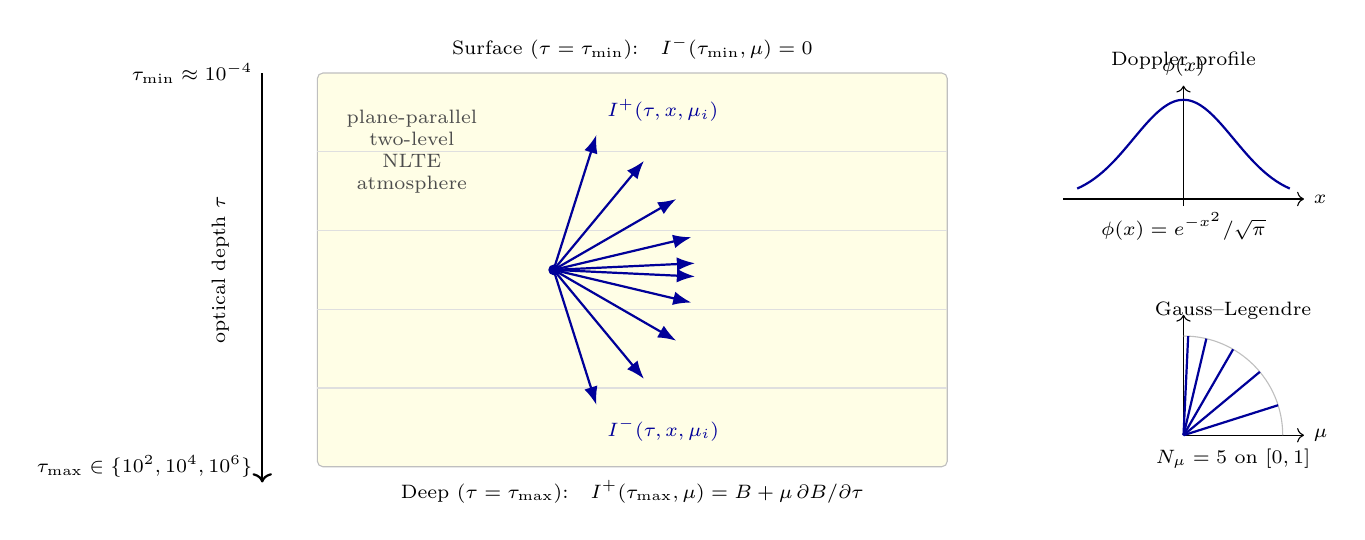
\begin{tikzpicture}[
  every node/.style={font=\footnotesize},
  ray/.style={-Latex, thick, blue!60!black},
]
% atmosphere slab
\filldraw[fill=yellow!10, draw=gray!50, rounded corners=2pt] (0,0) rectangle (8,5);

% depth grid lines (representative)
\foreach \y in {1,2,3,4} {
  \draw[gray!25, thin] (0,\y) -- (8,\y);
}

% boundary labels
\node[anchor=south, font=\scriptsize, align=center] at (4, 5.05)
  {Surface ($\tau = \tau_{\min}$):\quad$I^-(\tau_{\min}, \mu) = 0$};
\node[anchor=north, font=\scriptsize, align=center] at (4, -0.05)
  {Deep ($\tau = \tau_{\max}$):\quad$I^+(\tau_{\max}, \mu) = B + \mu\,\partial B/\partial \tau$};

% depth axis on the left
\draw[->, thick] (-0.7, 5) -- (-0.7, -0.2);
\node[font=\scriptsize, rotate=90, anchor=south] at (-1.0, 2.5) {optical depth $\tau$};
\node[anchor=east, font=\scriptsize] at (-0.7, 5) {$\tau_{\min} \approx 10^{-4}$};
\node[anchor=east, font=\scriptsize] at (-0.7, 0) {$\tau_{\max} \in \{10^2, 10^4, 10^6\}$};

% Ray fan from a single mid-depth point along the Gauss-Legendre directions.
% θ_i = arccos(μ_i) for the n_mu=5 default GL nodes on [0,1]:
%   μ = 0.0469, 0.2308, 0.5000, 0.7692, 0.9531
%   θ = 87.31°, 76.66°, 60.00°, 39.66°, 17.61°
% The ray direction in the figure (with surface = +y) is (sin θ, ±cos θ),
% i.e. polar angle ±(90° − θ) measured from +x.
\coordinate (raysrc) at (3, 2.5);
\filldraw[blue!60!black] (raysrc) circle (0.06);
\foreach \theta in {17.61, 39.66, 60.00, 76.66, 87.31} {
  \draw[ray] (raysrc) -- ++({90 - \theta}:1.8);   % I^+ (upward)
  \draw[ray] (raysrc) -- ++({\theta - 90}:1.8);   % I^- (downward)
}

\node[anchor=south west, font=\scriptsize, blue!60!black]
  at ($(raysrc) + ({90 - 17.61}:1.85)$) {$I^+(\tau, x, \mu_i)$};
\node[anchor=north west, font=\scriptsize, blue!60!black]
  at ($(raysrc) + ({17.61 - 90}:1.85)$) {$I^-(\tau, x, \mu_i)$};

% interior label
\node[font=\scriptsize, gray!60!black, align=center] at (1.2, 4.0)
  {plane-parallel\\two-level\\NLTE\\atmosphere};

% inset: line profile (top right)
\begin{scope}[shift={(11.0, 3.4)}, scale=0.9]
  \draw[->] (-1.7, 0) -- (1.7, 0) node[right, font=\scriptsize] {$x$};
  \draw[->] (0, -0.1) -- (0, 1.6) node[above, font=\scriptsize] {$\phi(x)$};
  \draw[blue!60!black, thick, smooth, samples=51, domain=-1.5:1.5]
    plot ({\x}, {1.4*exp(-\x*\x)});
  \node[font=\scriptsize, anchor=south, align=center] at (0, 1.7)
    {Doppler profile};
  \node[font=\scriptsize, anchor=north, align=center] at (0, -0.05)
    {$\phi(x) = e^{-x^2}/\sqrt{\pi}$};
\end{scope}

% inset: angle quadrature (lower right)
\begin{scope}[shift={(11.0, 0.4)}, scale=0.9]
  \draw[->] (0, 0) -- (1.7, 0) node[right, font=\scriptsize] {$\mu$};
  \draw[->] (0, 0) -- (0, 1.7);
  \draw[gray!50] (1.4, 0) arc[start angle=0, end angle=90, radius=1.4];
  \foreach \angle in {17.6, 39.7, 60.0, 76.7, 87.3} {
    \draw[blue!60!black, thick] (0,0) -- ({1.4*cos(\angle)}, {1.4*sin(\angle)});
  }
  \node[font=\scriptsize, anchor=south, align=center] at (0.7, 1.5)
    {Gauss--Legendre};
  \node[font=\scriptsize, anchor=north, align=center] at (0.7, -0.05)
    {$N_\mu = 5$ on $[0,1]$};
\end{scope}

\end{tikzpicture}
\caption{Schematic of the 1-D plane-parallel two-level NLTE testbed.
The depth coordinate $\tau$ runs from $\tau_{\min} \approx 10^{-4}$
(surface, top) to $\tau_{\max} \in \{10^2, 10^4, 10^6\}$ (deep, bottom);
the depth grid is logarithmic on $N_\tau = 80$ points by default.
The blue fan emanating from a representative mid-depth point shows the
five upgoing rays $I^+$ and five downgoing rays $I^-$ at the default
Gauss--Legendre $\mu$ angles (\,$\mu \in \{0.047, 0.231, 0.500, 0.769,
0.953\}$, equivalently $\theta = \arccos\mu \in
\{87.3^\circ, 76.7^\circ, 60.0^\circ, 39.7^\circ, 17.6^\circ\}$\,
from the local normal\,); the lower-right inset shows the same
quadrature on the unit semicircle.  Each ray is integrated by short
characteristics from depth to depth, and the mean intensity averages
over both half-spaces.  Boundary conditions: no incoming radiation at
the surface, and the diffusion-approximation form at depth
(Section~\ref{sec:bcs}), reducing exactly to $I^+ = B$ on isothermal
configurations.  The Doppler line profile $\phi(x) = e^{-x^2}/\sqrt{\pi}$
in dimensionless frequency offset $x = (\nu - \nu_0)/\Delta\nu_D$
(upper-right inset; default $N_\nu = 21$ on a half-width of $5$
Doppler widths) is integrated against $J(\tau, x)$ to form the
profile-weighted mean intensity $\Jbar(\tau)$.}
\label{fig:1d-setup}
\end{figure}

\subsection{The Line Source Function and Complete Redistribution}

For a two-level atom with no continuum, the line source function is
(HM14 §13.2)
\begin{equation}
S_l \;=\; \frac{n_2 A_{21}}{n_1 B_{12} - n_2 B_{21}}
\;=\; \frac{2 h \nu_0^3 / c^2}{n_1 g_2 / (n_2 g_1) - 1},
\label{eq:source-sl-pop}
\end{equation}
where the Einstein relations $A_{21} g_2 = (2 h \nu_0^3 / c^2) B_{21} g_2$
and $g_1 B_{12} = g_2 B_{21}$ have been used. In LTE (Boltzmann ratio), the
denominator becomes $\exp(h\nu_0 / kT) - 1$ and $S_l \to \Bnu(T)$.

Under CRD, the line source function admits the textbook two-level form
(HM14 §13.2; Avrett \& Hummer 1965):
\begin{equation}
\boxed{\; S_l \;=\; (1 - \epsilon)\,\Jbar + \epsilon\,B_\nu(T) \;}
\label{eq:S-eps}
\end{equation}
where $\Jbar$ is the line-profile-weighted mean intensity
\begin{equation}
\Jbar(\tau) \;\equiv\; \int \phi_\nu \, J_\nu(\tau)\, d\nu
\;=\; \int \phi(x)\, J(\tau, x)\, dx ,
\label{eq:Jbar}
\end{equation}
$J_\nu(\tau) = \tfrac{1}{2}\int_{-1}^{+1} I_\nu(\tau,\mu)\, d\mu$ is the
mean intensity, and $\epsilon$ is the photon destruction probability:
\begin{equation}
\epsilon \;\equiv\; \frac{C_{21}}{A_{21} + C_{21}}\!\left(1 - e^{-h\nu_0/kT}\right)^{-1}
\!\!\to\; \frac{C_{21}}{A_{21} + C_{21}}\quad(h\nu_0\!\ll\!kT)
\label{eq:eps}
\end{equation}
($C_{21}$ is the collisional de-excitation rate; the second form is the
textbook small-photon-energy approximation often quoted, e.g.,
HM14 eq.~13.29).  For the prototype, we treat $\epsilon$ as a free
parameter $\epsilon \in (0, 1]$ that controls how strongly the
atmosphere thermalizes the radiation: $\epsilon = 1$ is pure LTE, and
$\epsilon \to 0$ is pure scattering.

\subsection{The Lambda Operator}

The formal solution of equation~\eqref{eq:rte-tau-x-mu} for any prescribed
$S_l(\tau)$ is linear in $S_l$. Substituting into the definitions of
$J_\nu(\tau)$ and $\Jbar(\tau)$ yields a linear operator $\Lop$ acting on
$S_l$:
\begin{equation}
\Jbar(\tau) \;=\; (\Lop S_l)(\tau) \;=\; \int_0^{\tau_{\max}} K_1(|\tau - \tau'|)\, S_l(\tau')\, d\tau' ,
\label{eq:Lambda-op}
\end{equation}
where, for the CRD plane-parallel two-level problem with isotropic phase
function, the kernel $K_1$ has the explicit form (HM14 §13.3, eq.~13.50)
\begin{equation}
K_1(t) \;=\; \half\!\int\!\phi^2(x)\, E_1\!\left[\,\psi(x)\,t\,\right] dx ,
\label{eq:K1}
\end{equation}
with $E_1(x) = \int_1^\infty t^{-1} e^{-xt}\, dt$ the first exponential
integral. Combining \eqref{eq:S-eps} and \eqref{eq:Lambda-op} closes the
two-level CRD problem as the integral equation
\begin{equation}
S_l \;=\; (1-\epsilon)\, \Lop S_l + \epsilon\, B,
\label{eq:scattering-int-eq}
\end{equation}
which is the canonical scattering integral equation.
Equation~\eqref{eq:scattering-int-eq} is the workhorse: it admits the
Avrett--Hummer $\sqrt{\epsilon}$ surface law and the
$1/\sqrt{\epsilon}$ thermalization-depth result
(Section~\ref{sec:analytic-limits}).

Evaluating $\Lop$ numerically is what the \emph{formal solver} does.
Solving \eqref{eq:scattering-int-eq} numerically is what the
\emph{ALI driver} does (Section~\ref{sec:fixed-point}).

\subsection{Two-Level Statistical Equilibrium}
\label{sec:se-equations}

In statistical equilibrium $dn_i/dt = 0$, the population of each level
balances all radiative and collisional processes into and out of that
level.  For a two-level atom with no continuum, there is one
independent equation plus the closure $n_1 + n_2 = n_{\mathrm{tot}}$.
The rate balance is
\begin{equation}
n_1 \,(R_{12} + C_{12}) \;=\; n_2 \,(R_{21} + C_{21}),
\label{eq:rate-balance}
\end{equation}
with radiative rates (CRD: averaged over the line profile)
\begin{equation}
R_{12} \;=\; B_{12}\,\Jbar, \qquad
R_{21} \;=\; A_{21} + B_{21}\,\Jbar.
\label{eq:radiative-rates}
\end{equation}
Collisional rates obey detailed balance in LTE:
$C_{12} = (g_2/g_1)\,e^{-h\nu_0/kT}\, C_{21}$.

Solving \eqref{eq:rate-balance} together with the closure
$n_1 + n_2 = n_{\mathrm{tot}}$ yields a closed-form linear $2\times 2$ solve:
\begin{align}
\frac{n_2}{n_1} &= \frac{R_{12} + C_{12}}{R_{21} + C_{21}}, \label{eq:n2-over-n1}\\
n_1 &= \frac{n_{\mathrm{tot}}}{1 + n_2/n_1}, \quad n_2 = n_{\mathrm{tot}} - n_1.
\nonumber
\end{align}
This is the function the APNN emulator replaces.  It is the
\code{rate\_equation\_solve} function in
\code{atmosphere/rate\_equations.py}.

\subsection{Coupled Fixed-Point Structure}
\label{sec:fixed-point-structure}

The radiation field and the populations are mutually defined.  We
need $\Jbar$ to compute $(n_1, n_2)$ through SE, and we need $(n_1,
n_2)$ to compute $\Jbar$ through the formal solve and
\eqref{eq:source-sl-pop}.  This is a coupled fixed-point problem.

We define the \emph{reference coupled iteration operator} $\Tcyc$ ---
the cycle operator below, for brevity --- as one round of this
coupling:
\begin{equation}
\Tcyc(\mathbf{x}) \;=\; \Tse\bigl(\Trt(\mathbf{x})\bigr),
\label{eq:cycle}
\end{equation}
where the state vector $\mathbf{x}$ is the populations stacked over depth,
$\mathbf{x} \in \mathbb{R}^{N_\tau \times 2}$. The radiation step $\Trt$
maps populations to $\Jbar$ via \eqref{eq:source-sl-pop} and the formal
solve; the SE step $\Tse$ maps $\Jbar$ back to populations via
\eqref{eq:n2-over-n1}. The fixed point $\mathbf{x}^* = \Tcyc(\mathbf{x}^*)$ is
the converged NLTE state.  The qualifier ``reference'' distinguishes
$\Tcyc$ from the emulator-modified version $\Tcyc + \dT$ introduced
in \S\ref{sec:linearization}.

We define two variants:
\begin{itemize}
\item $\Tcyc_{\text{truth}}$: $\Tse$ is the closed-form rate-equation solver
of \eqref{eq:n2-over-n1}.
\item $\Tcyc_{\text{emul}}$: $\Tse$ is the APNN emulator.
\end{itemize}
The corresponding fixed points are $\mathbf{x}^*_{\text{truth}}$ and
$\mathbf{x}^*_{\text{emul}}$.  Their difference,
$\mathbf{x}^*_{\text{emul}} - \mathbf{x}^*_{\text{truth}}$, is the
\emph{converged} emulator error---the quantity GRAIL sets out to
predict from validation-set residuals.

Figure~\ref{fig:pipeline} shows the resulting end-to-end pipeline.
The reference cycle (green, top branch) and emulator cycle (orange, bottom
branch) share the radiation step $\Trt$ but diverge in the SE step;
their per-call difference is the residual $\dT$ that drives GRAIL.
GRAIL itself sits beneath the cycle.  It consumes the chain-rule JVP
$D\Tcyc\cdot\mathbf{v} = D\Tse(D\Trt\cdot\mathbf{v})$ through two
opaque callbacks (\code{host\_jvp} from $\Trt$, \code{emulator\_jvp}
from $\Tse$), takes the residual $\dT$ at the converged emulator
state, and solves the resolvent equation~\eqref{eq:resolvent}
matrix-free through GMRES.  GRAIL never imports either upstream
component; host-agnosticism is enforced by the callback signature.

\begin{figure}[ht]
\centering
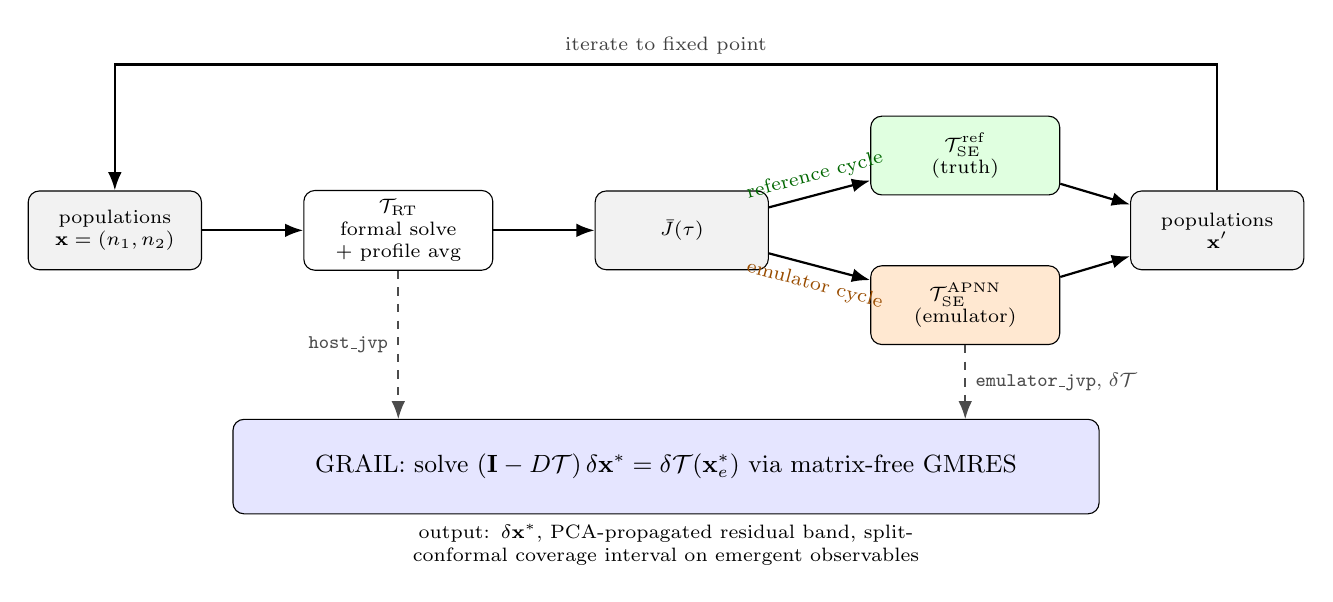
\begin{tikzpicture}[
  every node/.style={font=\footnotesize},
  state/.style={draw, rounded corners, fill=gray!10, minimum height=10mm, minimum width=22mm, align=center, font=\scriptsize},
  block/.style={draw, rounded corners, minimum height=10mm, minimum width=24mm, align=center, font=\scriptsize},
  truthblock/.style={block, fill=green!12},
  emulblock/.style={block, fill=orange!18},
  grailblock/.style={draw, rounded corners, fill=blue!10, minimum height=12mm, minimum width=110mm, align=center, font=\small},
  arr/.style={-Latex, thick},
  cb/.style={-Latex, thick, dashed, gray!60!black},
]
% top row: cycle
\node[state]      (x)      at (0,0)   {populations\\$\mathbf{x} = (n_1, n_2)$};
\node[block]      (Trt)    at (3.6,0) {$\Trt$\\formal solve\\$+$ profile avg};
\node[state]      (Jbar)   at (7.2,0) {$\Jbar(\tau)$};
\node[truthblock] (Ttruth) at (10.8,0.95) {$\Tse^{\mathrm{ref}}$\\(truth)};
\node[emulblock]  (Temul)  at (10.8,-0.95) {$\Tse^{\mathrm{APNN}}$\\(emulator)};
\node[state]      (xprime) at (14.0,0) {populations\\$\mathbf{x}'$};

\draw[arr] (x)      -- (Trt);
\draw[arr] (Trt)    -- (Jbar);
\draw[arr] (Jbar)   -- node[above, sloped, font=\scriptsize, green!40!black] {reference cycle} (Ttruth);
\draw[arr] (Jbar)   -- node[below, sloped, font=\scriptsize, orange!60!black] {emulator cycle} (Temul);
\draw[arr] (Ttruth) -- (xprime);
\draw[arr] (Temul)  -- (xprime);

% cycle feedback (iterate to fixed point); the +1.6 lift clears the truth
% block (Ttruth.north ≈ 1.45) so the horizontal segment runs above it.
\draw[arr] (xprime.north) -- ++(0,1.6) -| node[above, near start, font=\scriptsize, gray!50!black] {iterate to fixed point} (x.north);

% GRAIL block
\node[grailblock] (grail) at (7.0,-3.0) {GRAIL: solve $(\mathbf{I} - D\Tcyc)\,\delta\mathbf{x}^* = \dT(\mathbf{x}_e^*)$ via matrix-free GMRES};
\node[anchor=north, font=\scriptsize, align=center, text width=110mm] at (grail.south) {output: $\delta\mathbf{x}^*$, PCA-propagated residual band, split-conformal coverage interval on emergent observables};

% callbacks into GRAIL
\draw[cb] (Trt.south)   -- node[left,  font=\scriptsize] {\code{host\_jvp}} (3.6,-2.4);
\draw[cb] (Temul.south) -- node[right, font=\scriptsize] {\code{emulator\_jvp},\;$\dT$} (10.8,-2.4);
\end{tikzpicture}
\caption{The GRAIL pipeline.  Top row: the cycle
$\Tcyc = \Tse \circ \Trt$ iterates populations $\mathbf{x}$ through the
radiation step $\Trt$ (formal solve plus line-profile averaging) and
the SE step $\Tse$ to a fixed point.  $\Tse$ is the closed-form
rate-equation solver in the reference cycle (green) and the APNN in the
emulator cycle (orange); their per-call difference is the residual
$\dT$ that drives GRAIL.  Bottom: GRAIL consumes the chain-rule JVP
$D\Tcyc \cdot \mathbf{v} = D\Tse(D\Trt \cdot \mathbf{v})$ via two
opaque callbacks (\code{host\_jvp} from $\Trt$, \code{emulator\_jvp}
from $\Tse$) and the residual $\dT$ at the converged emulator state,
and solves the resolvent equation~\eqref{eq:resolvent} matrix-free via
GMRES.  GRAIL never imports either upstream component---host-agnosticism
is enforced by the callback signature.}
\label{fig:pipeline}
\end{figure}

\subsection{Photon Scattering and Thermalization in the Cycle Resolvent}
\label{sec:nlte-photon-scattering}

With the Lambda operator and the coupled fixed-point structure of the
NLTE problem now in hand, the abstract Methodology of
\S\ref{sec:methodology} acquires a concrete photon-physics reading.
For the two-level-atom CRD problem, the GRAIL Born
series~\eqref{eq:born-grail} reads as follows.  Each application of
$D\Tcyc$ is one full cycle of (1) populations modified by the
emulator residual, (2) source function $S_l$ recomputed via
\eqref{eq:source-sl-pop}, (3) radiation field $\bar{J}$ recomputed via
the formal solution, and (4) populations re-equilibrated by the
emulator's rate solve.  In line-formation language, this is one round
of \emph{radiative scattering plus rate-equation re-equilibration}: a
literal multiple-scattering event in the photon-scattering sense of
\S\ref{sec:lippmann-schwinger}, with the emulator residual playing the
role of the scattering potential.

The rate at which the GRAIL Born series converges is therefore governed
by the same physics that controls how a real photon thermalizes in a
scattering medium.  The Avrett--Hummer theorem
\citep{AvrettHummer1965}---developed in \S\ref{sec:avrett-hummer}
below---says that for an isothermal, semi-infinite, two-level CRD
atmosphere with photon destruction probability $\epsilon$, the surface source
function is $S_l(0)/B = \sqrt{\epsilon}$ and the thermalization length
is $\tau_{\mathrm{th}} \sim 1/\sqrt{\epsilon}$.  A photon emitted at
optical depth $\tau$ undergoes a random walk with
$\mathcal{O}(\epsilon^{-1})$ scattering events before being either
thermalized or escaping the surface.  In resolvent language, this
says the cycle operator has spectral radius $\rho(D\Tcyc) \to 1 -
\mathcal{O}(\epsilon)$ in the deep-medium, low-$\epsilon$ limit, so
the Born series converges geometrically at rate $1 -
\mathcal{O}(\epsilon)$, and summing it term by term takes $\sim
\epsilon^{-1}$ multiplications.  This is exactly why bare $\Lambda$
iteration stalls at low $\epsilon$ (\S\ref{sec:lambda-stall}): each
iteration is one term of the Born series.  GMRES on $(\mathbf{I} -
D\Tcyc)$ replaces the Avrett--Hummer random walk with a Krylov-subspace
construction whose iteration count grows sub-linearly with
$\epsilon^{-1}$, and is empirically governed by the condition number
of $D\Tcyc$ rather than its spectral radius (see the GMRES-scaling
row in \S\ref{sec:tests}).

The Eddington--Barbier surface relation $S_l(0) \approx J(\tau \!
\sim \! 1)$ is, in this language, a leading-order column of the cycle
Green's function $G \equiv (\mathbf{I} - D\Tcyc)^{-1}$: the response
at the surface to a unit thermal source near unit optical depth.  The
Avrett--Hummer $\sqrt{\epsilon}$ surface limit is the trace-norm-style
integral of $G$ across the medium.  Both analytic limits
(\S\ref{sec:analytic-limits}) are therefore direct probes of the same
Green's function whose discrete inverse GRAIL constructs.  The
testbed strategy of \S\ref{sec:1d-testbed}---verify against analytic
anchors before scaling---is the strategy of validating $G$ in the
limits where it is known in closed form.

% =============================================================================
\section{Application II: Self-Consistent Field Calculations in Electronic Structure}
\label{sec:scf-testbed}
% =============================================================================

The NLTE chapter just developed photon multiple scattering as the
physical content of the GRAIL Born series.  The same series describes
a coupled iteration that has nothing to do with photons.  We now show
this on the canonical self-consistent fixed-point problem of quantum
chemistry: the Hartree--Fock and Kohn--Sham self-consistent field (SCF)
iterations.  This is a second physical instantiation of GRAIL on the
same operator algebra, with a structurally different cycle and a
different physical interpretation of $\dT$, the cycle Jacobian, and
the amplification factor.

\subsection{Motivation: Neural Surrogates Inside the SCF Loop}
\label{sec:scf-motivation}

Hartree--Fock (HF) and Kohn--Sham (KS) density-functional theory
(DFT) have been the workhorses of electronic-structure calculation
for seventy years \citep{SzaboOstlund1996,ParrYang1989}.  Both
methods are self-consistent field (SCF) fixed-point iterations: the
electron density specifies the effective one-body Hamiltonian, the
Hamiltonian determines the orbitals, and the orbitals re-define the
density.  A converged calculation is by construction a fixed point
of the cycle that threads density $\rightarrow$ Fock matrix
$\rightarrow$ orbitals $\rightarrow$ density.

Within the last few years, neural surrogates for the
exchange--correlation (XC) functional have begun to enter that loop:
DM21 \citep{Kirkpatrick2021} learns a hybrid functional from
CCSD(T) reference data, and NeuralXC \citep{DickFernandezSerra2020}
learns correlation-consistent corrections to a baseline
density functional.
A user who substitutes such a surrogate for the conventional
B3LYP or PBE functional inside the SCF iteration has a per-call
residual against the truth functional at every encounter, and the
iteration re-injects that residual at every cycle until convergence.
This is exactly the coupled-iteration uncertainty problem of
\S\ref{sec:coupled-iter-problem}, expressed in electrons rather than
photons.  GRAIL's resolvent is therefore the natural object to
predict the converged-density error.  The question we ask is the same
one we asked for radiative transfer: given the per-call residual the
neural functional shows on a held-out test set, how much does the
self-consistent loop amplify it before the calculation halts?  And
when does that amplification become the dominant systematic in the
final density?

\subsection{The SCF Cycle as a Fixed-Point Composition}
\label{sec:scf-cycle}

One Roothaan--Hall iterate on the density matrix is the composition
of a Fock-build step and a diagonalize-and-rebuild step:
\begin{equation}
\Tcyc(\mathbf{P}) \;=\; \mathbf{D}\!\left[\mathbf{F}[\mathbf{P}]\right],
\qquad
\Tcyc \;=\; \mathbf{D} \circ \mathbf{F} ,
\label{eq:scf-cycle}
\end{equation}
which is the same compositional shape as
$\Tcyc = \Tse \circ \Trt$ in the NLTE chapter.  Here $\mathbf{P}$ is
the one-electron density matrix in an atomic-orbital basis; the
Fock-build map
\begin{equation}
\mathbf{F}[\mathbf{P}] \;=\;
\mathbf{h}_{\text{core}} + \mathbf{J}[\mathbf{P}] + \mathbf{V}_{\text{xc}}[\mathbf{P}]
\label{eq:scf-fock}
\end{equation}
assembles the effective one-body Hamiltonian as the sum of the
constant kinetic-plus-nuclear-attraction $\mathbf{h}_{\text{core}}$,
the Hartree--Coulomb matrix $\mathbf{J}[\mathbf{P}]$ (linear in
$\mathbf{P}$ via the two-electron integrals), and the
exchange--correlation matrix $\mathbf{V}_{\text{xc}}[\mathbf{P}]$
(nonlinear, and the slot where the neural surrogate replaces the
reference functional).  The diagonalize-and-rebuild map
\begin{equation}
\mathbf{D}[\mathbf{F}] \;=\;
2\,\mathbf{C}_{\text{occ}}\,\mathbf{C}_{\text{occ}}^{\top},
\qquad
\mathbf{F}\,\mathbf{C} \;=\; \mathbf{S}\,\mathbf{C}\,\boldsymbol\varepsilon,
\label{eq:scf-density}
\end{equation}
solves the generalized eigenproblem against the overlap
$\mathbf{S}$, takes the lowest $N/2$ occupied molecular orbitals
(closed shell), and projects them back into the density matrix.  The
converged density $\mathbf{P}^{*} = \Tcyc(\mathbf{P}^{*})$ is the SCF
solution; the per-call residual we will follow is the difference
$\delta\mathbf{V}_{\text{xc}} =
\mathbf{V}_{\text{xc}}^{\text{NN}} -
\mathbf{V}_{\text{xc}}^{\text{ref}}$, injected into
\eqref{eq:scf-fock} on every Fock build.

The composition $\mathbf{D} \circ \mathbf{F}$ matches GRAIL's chain-rule
callback API natively---no additive workaround is needed---which
makes SCF the cleanest cycle in our application set.  The NLTE cycle
threads radiation transport then statistical equilibrium; the SCF
cycle threads matrix construction then diagonalization.  GRAIL sees
both as two callbacks composed in series.

\subsection{The Cycle Jacobian: CPHF/CPKS as the SCF Analog of $\Lambda$}
\label{sec:scf-cphf}

The cycle Jacobian at the converged density factors by the chain
rule,
\begin{equation}
D\Tcyc\bigl|_{\mathbf{P}^{*}}
\;=\;
D\mathbf{D}\bigl|_{\mathbf{F}[\mathbf{P}^{*}]} \cdot
D\mathbf{F}\bigl|_{\mathbf{P}^{*}} ,
\label{eq:scf-DT-chain}
\end{equation}
and each factor has a name in the quantum-chemistry literature.  The
density-side factor $D\mathbf{D}$ is the noninteracting
density-matrix response $\chi_0$: working in the converged
molecular-orbital basis and applying first-order perturbation theory
to the projector onto occupied orbitals, the response of $\mathbf{P}$
to a perturbation in $\mathbf{F}$ is a sum over occupied--virtual
orbital pairs $(i, a)$, weighted by the inverse orbital-energy gap
$1/(\varepsilon_i - \varepsilon_a)$
\citep{Sternheimer1954,FurcheAhlrichs2002}.  The Fock-side factor
$D\mathbf{F}$ is the Hartree-plus-XC kernel $\mathbf{K} =
\partial(\mathbf{J} + \mathbf{V}_{\text{xc}})/\partial\mathbf{P}$.
The full cycle Jacobian is therefore
\begin{equation}
D\Tcyc\bigl|_{\mathbf{P}^{*}} \;=\; \chi_0\,\mathbf{K} ,
\label{eq:scf-DT-chi0K}
\end{equation}
which is the standard coupled-perturbed Hartree--Fock / Kohn--Sham
(CPHF / CPKS) response operator.  Sixty years of analytical-
derivative theory in quantum chemistry---geometry gradients,
magnetic susceptibilities, polarizabilities, NMR shifts---all
reduce to inverting precisely this operator
\citep{Pople1979,Helgaker2000}.

The structural analogy with the NLTE chapter is exact.  In the
two-level problem $D\Tcyc = (1-\epsilon)\Lop$: the Lambda operator
propagates a source through the medium, and $(1-\epsilon)$ converts
absorbed photons back into emitted ones.  In SCF, $\chi_0$ propagates
a Fock perturbation through the occupied--virtual orbital ladder, and
$\mathbf{K}$ converts a density change back into a Fock change.  The
two factors play structurally identical roles: $\chi_0$ is the SCF
analog of $\Lop$ (the propagator carrying a perturbation through the
matter--radiation coupling), and $\mathbf{K}$ is the SCF analog of
the $(1-\epsilon)$ rate-equation closure (the kernel converting the
propagated perturbation back into the cycle's input variable).  The
ALI preconditioner $\Lstar$ has its SCF counterpart too: in
quantum chemistry it is the diagonal-orbital-energy preconditioner
that the CPHF solver uses to invert $(1 - \chi_0\mathbf{K})$ at scale.
The operator algebra is the same algebra; only the physical
interpretation of the operators changes.

\subsection{The Amplification Regime: Approach to the Coulson--Fischer Instability}
\label{sec:scf-amplification}

What makes the SCF cycle amplify is not the HOMO--LUMO gap closing
through zero.  An expectation built on that picture turns out to be
empirically wrong on the closed-shell substrate, and the reason is
worth saying plainly because the right picture is more interesting.
In restricted Hartree--Fock (RHF) on stretched H$_2$, the dominant
eigenvalue of the cycle Jacobian $\chi_0\mathbf{K}$ is in fact
\emph{negative} along the orbital-rotation mode that mixes the
$\sigma_g$ HOMO with the $\sigma_u$ LUMO: the orbital-energy
denominator $\varepsilon_i - \varepsilon_a$ has one sign, the
Hartree-plus-XC kernel $\mathbf{K}$ has the other, and the resolvent
$(\mathbf{I} - \chi_0\mathbf{K})^{-1}$ stays bounded as $R$ grows.
The cycle's spectral content along the symmetry-preserving direction
is anti-amplifying, not amplifying.

The amplification that GRAIL is built to measure lives on a
\emph{different} mode of the same cycle, and is exposed only when the
substrate is unrestricted Hartree--Fock (UHF).  UHF carries an
independent set of $\beta$-spin orbitals; the cycle Jacobian gains
block structure
$\chi_0\mathbf{K} \to
(\chi_0^{\alpha}, \chi_0^{\beta}) \,
\mathbf{K}_{\alpha\beta}$,
and the new $\alpha$--$\beta$ off-diagonal block carries a
\emph{spin-localizing} mode absent from RHF.  As the bond stretches,
this mode's eigenvalue approaches $+1$ from below; at the
Coulson--Fischer point $R_{CF}$ it crosses through $+1$, the closed-
shell singlet ceases to be a stable solution of the UHF equations,
and a lower-energy broken-symmetry branch with $\alpha$ on one atom
and $\beta$ on the other becomes the variational minimum.  This is
the textbook \citet{CizekPaldus1967} triplet instability of
restricted Hartree--Fock; it is the open-shell content of every
bond-dissociation calculation; and it has the same Born-series shape
that drives photon multiple scattering toward thermalization in the
NLTE chapter.  Hartree--Fock stability analysis in its modern form
(\citealt{McWeeny1992,Helgaker2000}) is the systematic framework that
identifies it.

Near a regular solution, a positive cycle eigenvalue close to one can
produce a large response on the relevant physical tangent. DIIS can
accelerate convergence, but the derivative and residual used for response
must correspond to the unaccelerated physical cycle. State packing,
conservation constraints, and the norm used to report amplification are
part of the calculation.

The local response assumes that introducing the perturbation follows the
same smoothly varying regular solution. Comparing unrelated self-consistent
solutions is not justified by rescaling their prediction error. Nonlinear
remainder bounds depend on local derivatives and inverse norms; per-call
fit accuracy alone does not provide such a bound.

The runnable \code{examples/scf\_response.py} example verifies a controlled
family $F_\eta=F_t+\eta(F_{\rm NN}-F_t)$ at $\eta=10^{-3}$. It uses
independently converged reference and perturbed states, evaluates the
actual substituted Fock-to-density derivative at the perturbed state,
and checks both the linear equation defect and the measured density shift.
The family contains reference physics and tests local response rather
than production replacement or speedup.

\subsection{The Born Series for SCF}
\label{sec:scf-born}

Substituting \eqref{eq:scf-DT-chi0K} into the GRAIL resolvent
equation \eqref{eq:resolvent} gives the SCF Born series.  For a
per-call XC residual $\delta\mathbf{V}_{\text{xc}}(\mathbf{P}^{*})$,
\begin{equation}
\delta\mathbf{P}^{*}
\;=\;
\bigl(\mathbf{I} - \chi_0\,\mathbf{K}\bigr)^{-1} \chi_0\,
\delta\mathbf{V}_{\text{xc}}(\mathbf{P}^{*})
\;+\; \mathcal{O}\!\left(\|\delta\mathbf{V}_{\text{xc}}\|^{2}\right) ,
\label{eq:scf-resolvent}
\end{equation}
and the geometric expansion of the resolvent gives the term-by-term
expansion
\begin{equation}
\delta\mathbf{P}^{*}
\;=\;
\chi_0\,\delta\mathbf{V}_{\text{xc}}
\;+\;
\chi_0\,\mathbf{K}\,\chi_0\,\delta\mathbf{V}_{\text{xc}}
\;+\;
(\chi_0\,\mathbf{K})^{2}\,\chi_0\,\delta\mathbf{V}_{\text{xc}}
\;+\; \cdots .
\label{eq:scf-born}
\end{equation}
The leading term is the bare orbital-relaxation response: the
density change a held-out test set would predict if the SCF loop
were a single Sternheimer call.  Each subsequent term inserts one
more pair of vertices on the Feynman diagram: a propagation through
the orbital ladder ($\chi_0$) followed by a kernel-induced
re-build of the Fock matrix ($\mathbf{K}$).  In multiple-scattering
language each $\chi_0\mathbf{K}$ application is one round trip of
orbital relaxation chased by Hartree-and-XC re-evaluation.  In
chemistry language each application is one CPKS iteration.  In
GRAIL's language it is one cycle of the loop, and the resolvent
sums them all.

The series and the matrix inverse are the same object, just written
differently.  GRAIL evaluates~\eqref{eq:scf-resolvent} the same way
it does in NLTE: matrix-free GMRES on $(\mathbf{I} -
\chi_0\mathbf{K})$, with $\chi_0\mathbf{K} \cdot \mathbf{v}$ supplied
through composed callbacks.  The two callbacks have a labeling
caveat that does not arise in NLTE: the chain rule applies
$D\mathbf{F}$ first and $D\mathbf{D}$ second, so the slot named
\code{host\_jvp} in the GRAIL API corresponds to $D\mathbf{F}$ here
(the Fock-build block, which is where the neural functional lives),
and \code{emulator\_jvp} corresponds to $D\mathbf{D}$ (the
neural-functional-free diagonalize step).  The label
``emulator\_jvp'' reflects the chain-rule position, not the location
of the neural component.

The derivative must pass through the actual neural Fock contribution
used in the iteration. Forward-mode automatic differentiation provides
this derivative; an independent finite-difference check can diagnose
implementation and step-size errors. Substituting a derivative of the
reference functional changes the operator and does not propagate the
same surrogate perturbation. The runnable SCF example checks the
predicted shift and the true linear equation defect independently.


\subsection{Physical Settings Where the Stretched-Bond Regime Lives}
\label{sec:scf-physical-settings}

Stretched H$_2$ at $2$--$3 R_{\text{eq}}$ is a textbook example, but
it is not academic: the same near-multireference regime appears in
real physical and astrophysical settings whenever a bond is sampled
far from its equilibrium length.  Photodissociation of molecular
hydrogen in photodissociation regions and protostellar disks
populates the entire reaction coordinate from $R_{\text{eq}}$ to the
asymptote, and the calculation of the dissociation cross section
requires accurate energies all the way through the stretched-bond
regime.  Thermal dissociation of H$_2$ in the atmospheres of M
dwarfs, brown dwarfs, and hot Jupiters traverses the same coordinate
on a temperature axis: the molecular fraction of hydrogen in such
atmospheres is set by an equilibrium constant that depends on the
electronic energy at every $R$.  Even at room temperature, the
zero-point and thermal vibrational sampling of H$_2$ extends well
into the slow-SCF regime; molecular-dynamics calculations that build
in those samples encounter stretched-bond points routinely.
H-abstraction reaction barriers in combustion and biochemistry pass
through transition states with one bond stretched and another
forming, again sampling the near-multireference regime by
construction.

Each of these settings is a use case where the per-call accuracy a
neural XC functional reports on its training distribution
\emph{undersells} the converged-density error a user sees in
production.  The cycle approaches a Coulson--Fischer-style
instability somewhere along the reaction coordinate; the cycle
amplifies; the held-out validation residual is the leading-order
term of a Born series with many more terms behind it.  GRAIL is the
machinery for measuring how many.

\subsection{Connection to Published Implicit-Differentiation Work in SCF}
\label{sec:scf-related-work}

The closest published precedent for the present chapter is
\citet{Schmitz2025}, which implements implicit automatic
differentiation
through the SCF fixed point in DFTK to propagate input-parameter
uncertainty into converged-density observables.  The resolvent
operator $(\mathbf{I} - \chi_0\mathbf{K})^{-1}$ is the same operator
they invert; their solver is structurally identical to GRAIL's
matrix-free GMRES on the SCF cycle Jacobian.  GRAIL uses implicit response to propagate an operator-replacement residual
through opaque host and neural callbacks. Its separate conformal calibrator
applies to a declared prediction target when the exchangeability assumptions
hold; an executable calibration example does not establish production SCF
coverage. The core solver imports no electronic-structure package.
Set
against the broader sixty-year history of CPHF, CPKS, the Sternheimer
equation, and density-functional perturbation theory
\citep{Baroni2001}, all of which invert the same response operator
for physical perturbations (geometries, fields, phonon
displacements), the present application is the first to use that
operator on ML-surrogate residuals in coupled iteration.

% =============================================================================
\section{GRAIL Architecture}
\label{sec:resolvent}
% =============================================================================

The mathematical content of GRAIL---the resolvent equation, its
Green's-function structure, and its connection to Lambda-ALI scattering
theory---is laid out in Section~\ref{sec:methodology}.  This section
covers the practical architecture: the structural commitments that
shape the library's API, and the callback discipline that makes the
resolvent solve host-code-agnostic.

\subsection{Structural Commitments}

The structural commitments of GRAIL are:
\begin{itemize}
\item \textbf{Host-code-agnostic.}  The GRAIL driver consumes the
emulator JVP and the host JVP as opaque callbacks.  The same library
wraps a PyTorch-native prototype (this work) or a Fortran legacy code
(the eventual future-work \textsc{thornado}/\textsc{Flash-X} integration).
\item \textbf{Matrix-free.}  The cycle differential is never
assembled.  Each GMRES iteration costs one emulator JVP plus one host
JVP.
\item \textbf{PCA $+$ conformal.}  Validation residuals are decomposed
by truncated SVD; each principal component is propagated through the
resolvent independently.  A split-conformal calibrator on the residual
band delivers finite-sample distribution-free coverage on
observables.
\end{itemize}

\subsection{Composing Through Callbacks}

The chain rule \eqref{eq:cycle-chainrule} applied to a vector $\mathbf{v}$
gives
\begin{equation}
D\Tcyc \cdot \mathbf{v} \;=\; D\Tse \cdot (D\Trt \cdot \mathbf{v}).
\end{equation}
GRAIL evaluates this through two callbacks.  The
\texttt{emulator\_jvp(v)} callback computes $D\Tse \cdot \mathbf{v}$
through PyTorch \code{torch.func.jvp}.  The \texttt{host\_jvp(v)}
callback computes $D\Trt \cdot \mathbf{v}$ the same way (or, in the
eventual \textsc{thornado}/\textsc{Flash-X} adaptor, through a Fortran
adjoint).  The matrix-vector product that GMRES solves is
\begin{equation}
\mathbf{v} \;\mapsto\; \mathbf{v} - D\Tcyc \cdot \mathbf{v}
\;=\; \mathbf{v} - \mathtt{emulator\_jvp}(\mathtt{host\_jvp}(\mathbf{v})).
\label{eq:matvec}
\end{equation}
This is the host-agnosticism property of GRAIL: nothing in
\eqref{eq:matvec} requires the GRAIL driver to know what either
callback is doing inside.  It can be PyTorch-on-PyTorch (this
prototype), a PyTorch emulator wrapping a Fortran formal solver (the
eventual integration target), or anything else.  The honesty test
(docs/testing.md \texttt{I-callback-isolation}) checks that GRAIL runs to
completion when given a callback that \emph{hides} PyTorch from it
(for example, a NumPy-array-in/-out wrapper).

It is worth heading off a possible source of confusion here.  GRAIL is
host-\emph{agnostic}, not host-\emph{independent}.  The resolvent
solve manifestly needs the host's Jacobian action $D\Trt \cdot
\mathbf{v}$; without it, $D\Tcyc$ has no second factor and
\eqref{eq:matvec} cannot be evaluated.  ``Host-agnostic'' means only
that this dependence is funneled entirely through the callback API.
The GRAIL package \code{grail/} contains no \code{import atmosphere}
or \code{import emulator} statement---enforced by structure and
verified by \texttt{I-callback-isolation}---and the same GRAIL binary
works unchanged across hosts that supply a conforming
\texttt{host\_jvp}.  The host is connected to GRAIL at \emph{API
time} (when the caller passes \texttt{host\_jvp} into
\code{resolvent\_solve}), not at \emph{import time}.  The two notions
are distinct, and only the import-time dependence is what GRAIL has
eliminated.  The runtime dependence on the host's Jacobian is a
feature, not a bug.

\subsection{Backend Choice}
\label{sec:backend-choice}

GRAIL supports PyTorch and JAX. The dispatch function is
\code{grail.backend.get\_backend(...)}.
Forward-mode automatic differentiation through the emulator is
provided by \code{torch.func.jvp} on the PyTorch backend and
\code{jax.jvp} on the JAX backend, with both filling the
\texttt{emulator\_jvp} slot through the same opaque callback
contract.  The two backends share the public entry point
\code{resolvent\_solve} and the same \texttt{host\_jvp} /
\texttt{emul\_jvp} signatures, so a JAX-native host code that supplies
a conforming pair runs through GRAIL without round-tripping its state
through PyTorch, and conversely.  Backend selection is a runtime
configuration choice rather than a compile-time commitment.  The backend tests exercise their array and linear-algebra contracts,
and a JAX response solve checks the retained backend independently.
Backend-specific compilation and
preconditioning costs should be measured for the intended host and state size.

% =============================================================================
\section{Analytic Limits}
\label{sec:analytic-limits}
% =============================================================================

The analytic tests described in \code{docs/testing.md} are not arbitrary numerical sanity checks.
They are the four limits in which the two-level CRD problem has a known
closed-form (or asymptotic) solution.  Agreement to within a percent-level
tolerance is what separates a host that is correct from one that is merely
\emph{running}.

\subsection{The Eddington--Barbier Relation}
\label{sec:eddington-barbier}

\textbf{Statement.} For an atmosphere in which $S_l(\tau)$ varies linearly
with optical depth, $S_l(\tau) = a + b\tau$, the surface emergent intensity
in direction $\mu$ is
\begin{equation}
I(0, \mu) \;=\; a + b\mu \;=\; S_l(\tau = \mu).
\label{eq:eddington-barbier}
\end{equation}
In words: the surface intensity in any given direction is approximately
the local source function at $\tau = \mu$.  Look one mean free path down
along the ray, and you read off the radiation that comes out.  (HM14
§11.5; M78 §2-3.)

\textbf{Derivation.} Integrating the formal solution of
\eqref{eq:rte-tau-x-mu} for an upgoing ray ($\mu > 0$) in a semi-infinite
atmosphere with vanishing inflow at depth, the emergent intensity at the
surface ($\tau = 0$) at line center ($\psi = 1$) is
\begin{equation}
I(0, \mu) \;=\; \int_0^{\infty} S_l(\tau)\, e^{-\tau/\mu}\, \frac{d\tau}{\mu}.
\label{eq:emergent-int}
\end{equation}
Substituting $S_l(\tau) = a + b\tau$:
\begin{align}
I(0, \mu)
&= \frac{1}{\mu}\!\left[ a\!\int_0^\infty\! e^{-\tau/\mu}\,d\tau + b\!\int_0^\infty\! \tau\, e^{-\tau/\mu}\,d\tau\right]\\
&= \frac{1}{\mu}\!\left[ a\,\mu + b\,\mu^2\,\Gamma(2) \right] = a + b\mu .
\end{align}
This is the standard exponential-integral evaluation; the gamma-function
factor $\Gamma(2) = 1$ comes from $\int_0^\infty \tau\, e^{-\tau/\mu}\,d\tau = \mu^2$.

\textbf{Test gating.} docs/testing.md \texttt{A-eddington-01} feeds a linear $S$
into the formal solver and checks that $I(0, \mu) = a + b\mu$ to within
$5\%$ at $\mu \in \{0.1, 0.5, 0.9\}$.  The test does not require iteration
(no rate equations, no fixed point); it is purely a formal-solver gate.
A formal solver that fails Eddington--Barbier is wrong somewhere in its
characteristic integration or its boundary handling.

\subsection{The Avrett--Hummer Thermalization Theorem}
\label{sec:avrett-hummer}

\textbf{Statement.} For an isothermal semi-infinite atmosphere with constant
$\epsilon$ and Doppler line profile, the line source function obeys (HM14
§13.3, originally Avrett \& Hummer 1965):
\begin{enumerate}[label=(\roman*)]
\item Surface value: $S_l(0) / B = \sqrt{\epsilon}$, modulo logarithmic
factors of the line profile.
\item Thermalization depth: $S_l(\tau)/B \to 1$ as $\tau \to \tau_{\text{therm}}$
where $\tau_{\text{therm}} \sim 1/\sqrt{\epsilon}$ for Doppler profiles
(strictly, $\tau_{\text{therm}} \approx 1/(\sqrt{\pi}\,\epsilon)$ for the
Holstein single-flight approximation; the Doppler-profile version differs by
a logarithmic factor and is plotted in HM14 Fig.~13.4).
\end{enumerate}

\textbf{Origin of the $\sqrt{\epsilon}$ scaling.}  The picture is a
photon doing a random walk against the prospect of being killed.  In a
two-level scattering atmosphere a photon undergoes on average
$1/\epsilon$ scatterings before it is thermalized---destroyed by
collisional de-excitation with probability $\epsilon$ per scattering.
Each scattering displaces the photon by roughly one mean free path.
The number of scatterings scales as $1/\epsilon$, and for a random
walk with step size of order unity in optical depth the
root-mean-square displacement is $\sqrt{N_{\text{scatt}}} =
1/\sqrt{\epsilon}$.  So a photon born at optical depth $\tau \gtrsim
1/\sqrt{\epsilon}$ is thermalized before it can escape, and the source
function thermalizes at that depth.  The escape probability of a
photon born at the surface is $\sim \sqrt{\epsilon}$; hence
$S_l(0) / B \sim \sqrt{\epsilon}$.

\textbf{Test gating.} docs/testing.md \texttt{A-thermalization-01} checks that
$S_l(\tau = 1/\sqrt{\epsilon})/B \in [0.5, 1.0]$ for
$\epsilon \in \{10^{-2}, 10^{-4}, 10^{-6}\}$; \texttt{A-thermalization-02}
checks $S_l(0)/B = \sqrt{\epsilon}$ to within $10\%$ across the same range.
These are the anchor physics-correctness tests of the host.  A failure
in either points to a fundamental error in the formal solver, the line
profile averaging, or the ALI driver.

\subsection{The LTE Limit}

\textbf{Statement.} As $\epsilon \to 1$, the two-level CRD problem reduces to
LTE: $S_l \to B$ at all depths, and the populations follow the Boltzmann
ratio $n_2 / n_1 = (g_2/g_1) \exp(-h\nu_0/kT)$.

\textbf{Derivation.} From \eqref{eq:S-eps}, $S_l \to B$ as $\epsilon \to 1$.
Substituting into \eqref{eq:source-sl-pop} and using the Einstein relations,
$2 h\nu_0^3/c^2 = (n_1 g_2 / n_2 g_1 - 1)\, B \to (n_1 g_2 / n_2 g_1 - 1)\, \Bnu(T)$.
Solving for $n_2 / n_1$ recovers the Boltzmann ratio.

\textbf{Test gating.} \texttt{A-lte-01} checks that $S_l \to B$ at
every depth and that the converged populations are Boltzmann to
$10^{-6}$.  Convergence in a single iteration of ALI is a useful
sub-check (test \texttt{U-fixedpoint-01}): at $\epsilon = 1$ the
iteration \eqref{eq:ali-iter} immediately yields $S_l = B$, and a
correct ALI driver should hit that answer in one step.

\subsection{The Coherent Two-Stream Limit}
\label{sec:coherent-twostream}

\textbf{Statement.} In the limit of coherent monochromatic scattering---i.e.,
the line profile collapses to a delta function $\phi(x) \to \delta(x)$, and
the radiation field is described at a single frequency---the two-level
scattering problem with isotropic phase function reduces to the classical
Schwarzschild--Milne integral equation, which admits the analytic two-stream
(Eddington-approximation) solution
\begin{equation}
S_l(\tau) \;=\; B\!\left[\,1 - (1 - \sqrt{\epsilon})\,e^{-\sqrt{3\epsilon}\,\tau}\,\right]
\quad \text{(two-stream)}.
\label{eq:two-stream}
\end{equation}
(M78 §6-3, eq.~6-39; HM14 §13.3 reviews this for context.) The surface value
is $S_l(0) = \sqrt{\epsilon}\, B$, recovering the Avrett--Hummer
$\sqrt{\epsilon}$ result; the thermalization depth in this limit is
$1/\sqrt{3\epsilon}$.

\textbf{Test gating.} \texttt{A-coherent-01} runs the prototype in a
single-frequency setup ($N_\nu = 1$, $\phi = 1$, $\psi = 1$) and checks
agreement with \eqref{eq:two-stream} to $\sim 5\%$ at the same set of
$\epsilon$ values.  This test exercises the full
ALI-formal-solver-rate-equation loop in a regime where the answer is
known in closed form, without the line-profile integration contributing
to the numerical error.

% =============================================================================
\section{Numerical Discretization}
\label{sec:discretization}
% =============================================================================

\subsection{Optical Depth Grid}
\label{sec:depth-grid}

The depth grid is logarithmic in line-center optical depth:
\begin{equation}
\tau_i \;=\; \tau_{\min}\!\left(\frac{\tau_{\max}}{\tau_{\min}}\right)^{i/(N_\tau-1)},
\qquad i = 0, \ldots, N_\tau - 1.
\end{equation}
Logarithmic spacing reflects the multiplicative structure of the
radiation problem: photon escape probability and thermalization both
scale logarithmically with $\tau$.  Default values per SPEC §3.1 are
$\tau_{\min} = 10^{-4}$ (formally surface; this resolves the
Eddington--Barbier limit), $\tau_{\max} \in \{10^2, 10^4, 10^6\}$,
$N_\tau = 80$.

We use float64 throughout, and double precision is not gratuitous
here.  At $\epsilon = 10^{-6}$ the $\sqrt{\epsilon}$ surface value is
$10^{-3}$, and \texttt{A-thermalization-02} requires reproducing this
to within $10\%$ relative---an additive error of $10^{-4}$ in $S/B$.
Single-precision rounding errors of order $10^{-7}$ accumulating over
$\mathcal{O}(10^4)$ ALI iterations would walk right up to that
tolerance.  Double precision keeps a five-decade safety margin.

\textbf{Implementation.} \code{atmosphere/grid.py} provides
\code{DepthGrid.log\_spaced(tau\_min, tau\_max, n\_tau)}, which returns a
\code{DepthGrid} dataclass holding a 1-D \code{torch.Tensor tau} of shape
\code{(n\_tau,)}, dtype \code{float64}. The Tier~U test
\texttt{U-grid-01} verifies monotonicity, log-spacing (constant ratio
$\tau_{i+1}/\tau_i$), and exact endpoint matching, all to relative
tolerance $10^{-12}$.

\subsection{Frequency Grid}
\label{sec:freq-grid}

The frequency grid is dimensionless: $x = (\nu - \nu_0)/\Delta\nu_D$ on
the interval $[-x_{\max}, x_{\max}]$, with $x_{\max} = 5$ by default. The
nodes are uniformly spaced. The line profile values are stored explicitly:
$\phi(x) = e^{-x^2}/\sqrt{\pi}$. Integration weights are trapezoidal:
$w_i = \Delta x$ for interior points, $w_0 = w_{N_\nu - 1} = \Delta x / 2$
for endpoints, with $\Delta x = 2 x_{\max}/(N_\nu - 1)$.

The line-profile-weighted mean intensity in the discrete representation is
\begin{equation}
\Jbar(\tau) \;\approx\; \sum_{i=0}^{N_\nu - 1} w_i \,\phi(x_i)\, J(\tau, x_i).
\label{eq:Jbar-discrete}
\end{equation}
The docs/testing.md gate \texttt{U-grid-02} requires
$\sum_i w_i \,\phi(x_i) = 1$ to $10^{-10}$.

\subsubsection{Trapezoidal Convergence on Gaussians}

The trapezoidal rule has a conventional reputation for second-order
convergence on smooth functions, but for analytic functions on the
real line it is in fact exponentially convergent
\citep{TrefethenWeideman2014}.  The truncation error of the
trapezoidal sum
\begin{equation}
T_h[f] \;=\; h \sum_{n=-\infty}^{+\infty} f(n h)
\end{equation}
applied to a function $f$ analytic in a strip of half-width $a$ around
the real axis decays as $|T_h[f] - \int f| \lesssim e^{-2\pi a / h}$.
For the Gaussian $f(x) = e^{-x^2}$, $a$ is unbounded; the trapezoidal
rule on the infinite real line therefore gives essentially exact
integration as soon as $h$ is of order unity.

Truncating the integral to a finite interval $[-x_{\max}, x_{\max}]$
adds a tail contribution
\begin{equation}
\Delta_{\text{tail}} \;=\; 2 \int_{x_{\max}}^\infty \frac{e^{-x^2}}{\sqrt{\pi}}\, dx
\;=\; \mathrm{erfc}(x_{\max}).
\end{equation}
For $x_{\max} = 5$, $\mathrm{erfc}(5) \approx 1.5 \times 10^{-12}$,
well below the $10^{-10}$ tolerance.  At default settings ($N_\nu =
21$, $x_{\max} = 5$) the realized error is $\sim 10^{-12}$, comfortably
inside spec.

\textbf{Implementation.} \code{FrequencyGrid.doppler(n\_nu=21, half\_width=5.0)}
returns a dataclass holding three \code{(n\_nu,)} tensors: \code{nu} (the
$x_i$, abusing notation to align with SPEC), \code{weights} (the trapezoidal
$w_i$), \code{profile} (the $\phi(x_i)$).

\subsection{Angular Quadrature}
\label{sec:angle-quad}

In plane-parallel geometry we exploit reflection symmetry: rays
propagate upward ($\mu > 0$) or downward ($\mu < 0$), and the formal
solver treats each half-space separately.  We store positive $|\mu|$
only and use the same nodes and weights for both directions.

The chosen quadrature is $N_\mu$-point Gauss--Legendre on $[0, 1]$,
obtained from the standard Gauss--Legendre quadrature on $[-1, 1]$
via the affine transformation $\mu = (\xi + 1)/2$, $w_\mu = w_\xi / 2$.
With this normalization $\sum_i w_i = 1$, matching $\int_0^1 d\mu = 1$.
The mean intensity reduces to
\begin{equation}
J(\tau, x) \;=\; \half\!\sum_{i=0}^{N_\mu - 1} w_i\!\left[\,I^{+}(\tau, x, \mu_i) + I^{-}(\tau, x, \mu_i)\,\right].
\label{eq:J-discrete}
\end{equation}

$N$-point Gauss--Legendre integrates polynomials of degree $\leq 2N - 1$
exactly.  The default $N_\mu = 5$ therefore integrates polynomials of
degree $\leq 9$ exactly, well past the $\mu^k$ for $k \in \{0,1,2,3\}$
that the Tier~U test \texttt{U-grid-03} exercises.

\textbf{Implementation.} \code{AngleQuadrature.gauss\_legendre(n\_mu=5)} uses
\code{numpy.polynomial.legendre.leggauss} to obtain $\xi_i, w_{\xi,i}$ on
$[-1, 1]$, then converts to torch float64 tensors after the affine
transformation.

\subsection{Boundary Conditions}
\label{sec:bcs}

The semi-infinite plane-parallel atmosphere is truncated at $\tau_{\max}$.
The boundary conditions are:
\begin{itemize}
\item \textbf{Surface} ($\tau = \tau_{\min} \approx 0$): no incoming
radiation from above, $I^{-}(\tau_{\min}, \mu) = 0$ for all $\mu \in [0, 1]$
(downgoing rays at the top of the atmosphere).
\item \textbf{Deep} ($\tau = \tau_{\max}$): diffusion (first-order Eddington)
boundary condition for upgoing rays:
\begin{equation}
I^{+}(\tau_{\max}, \mu) \;=\; B(T(\tau_{\max})) + \mu\,\frac{\partial B}{\partial \tau}\bigg|_{\tau_{\max}} .
\label{eq:lower-bc}
\end{equation}
\end{itemize}

For an isothermal atmosphere (the canonical test config),
$\partial B/\partial \tau = 0$ and \eqref{eq:lower-bc} reduces to
$I^+ = B$, exact in the diffusion limit.  The diffusion form
generalizes cleanly to the power-law $T(\tau)$ canned config without
forcing a deeper $\tau_{\max}$ to suppress BC bleed-through.  (HM14
§11.6 derives the diffusion BC as the leading-order asymptotic of the
formal solution at $\tau \gg 1$.)

\subsection{Tensor Conventions}

All computations use \code{torch} float64 tensors with the following shape
conventions inside \code{atmosphere/}:

\begin{center}
\begin{tabular}{@{}lll@{}}
\toprule
Quantity & Shape & Notes \\ \midrule
$\tau$ & \code{(n\_tau,)} & log-spaced, ascending from surface \\
$x$, $\phi$, $w$ & \code{(n\_nu,)} & symmetric around line center \\
$\mu$, $w_\mu$ & \code{(n\_mu,)} & Gauss--Legendre on $[0, 1]$ \\
$T$, $n_e$, $\Jbar$, $S_l$ & \code{(n\_tau,)} & per-depth scalars \\
$J(\tau, x)$, $S(\tau, x)$ & \code{(n\_tau, n\_nu)} & monochromatic; CRD: $S(\tau,x)\!=\!\Sl(\tau)$ \\
$(n_1, n_2)$ & \code{(n\_tau, 2)} & populations; output of \code{rate\_equation\_solve} \\
state $\mathbf{x}$ & \code{(n\_tau, 2)} & inside \code{atmosphere/} \\
state at GRAIL seam & \code{(2 * n\_tau,)} & flat blocked: \code{populations.T.flatten()} \\
\bottomrule
\end{tabular}
\end{center}

The flattening to a 1-D state vector happens only at the GRAIL
boundary, in \code{grail/jacobian.py}, because Krylov methods natively
want 1-D vectors.  The blocked layout (all $n_1$ values, then all
$n_2$ values) preserves depth-coherence for cache-friendly per-depth
operations.  The interleaved layout, \code{populations.flatten()} from
a \code{(n\_tau, 2)} tensor, would scramble depth and is exactly what
we are avoiding.

% =============================================================================
\section{The Formal Solver}
\label{sec:formal-solver}
% =============================================================================

\subsection{The Short-Characteristics Method}

The formal-solution problem is this: given $S_l(\tau)$ on the depth
grid, compute $J(\tau, x) = (1/2) \sum_i w_i [I^+(\tau, x, \mu_i) +
I^-(\tau, x, \mu_i)]$ at each $(\tau_j, x_k)$.  The short-characteristics
(SC) method (\citep{Olson1987}; HM14 §11.4) integrates the RTE along
each characteristic ray segment by segment, between consecutive depth
grid points.  This is in contrast to long characteristics, which
integrate the full ray from the relevant boundary in one shot.  We
prefer SC for its $\mathcal{O}(N_\tau)$ scaling per ray (versus
$\mathcal{O}(N_\tau^2)$ for LC); both methods have identical accuracy
at fixed depth resolution under linear interpolation of $S$.

For an upgoing ray ($\mu > 0$) the integration sweeps from the lower
boundary $\tau_{\max}$ to the surface $\tau_{\min}$; for a downgoing
ray ($\mu < 0$, stored with the same $|\mu|$ in our convention) the
sweep reverses.

\subsection{Linear Source-Function Interpolation}

Within a single depth segment $[\tau_a, \tau_b]$ with $\tau_a < \tau_b$,
linear interpolation of the source function in optical depth gives
\begin{equation}
S(\tau) \;=\; S_a + (S_b - S_a)\,\frac{\tau - \tau_a}{\Delta\tau},
\qquad \Delta\tau \equiv \tau_b - \tau_a.
\end{equation}
For an upgoing ray at angle $\mu > 0$ at frequency $x$, the optical-depth
increment along the path is $\Delta\tau_\nu = \psi(x)\,\Delta\tau$ in the
direction of propagation, and the formal-solution increment is
\begin{equation}
I_b \;=\; I_a\, e^{-u} + \int_0^{u}\!\!S(s)\, e^{-(u-s)}\,ds,
\qquad u \equiv \frac{\psi(x)\,\Delta\tau}{\mu} .
\label{eq:sc-integral}
\end{equation}

\subsection{The Olson--Kunasz Coefficients: Derivation}
\label{sec:ok87}

Substituting the linear-in-optical-depth $S$ into \eqref{eq:sc-integral},
\begin{align}
I_b - I_a\, e^{-u}
&= \int_0^u \!S_a e^{-(u-s)}\, ds + \int_0^u\! \frac{S_b - S_a}{u}\, s\, e^{-(u-s)}\, ds\\
&= S_a\,(1 - e^{-u}) + \frac{S_b - S_a}{u}\,\!\!\int_0^u\! s\, e^{-(u-s)}\, ds.
\label{eq:ok87-step1}
\end{align}
The remaining integral is, after substituting $t = u - s$:
\begin{equation}
\int_0^u\! s\, e^{-(u-s)}\, ds \;=\; \int_0^u (u - t)\, e^{-t}\, dt
\;=\; u\,(1 - e^{-u}) - \!\int_0^u\! t\, e^{-t}\, dt.
\end{equation}
The last integral is $1 - (1 + u) e^{-u}$ by integration by parts:
$\int t\, e^{-t}\, dt = -(t+1)e^{-t}$. Hence
\begin{equation}
\int_0^u\! s\, e^{-(u-s)}\, ds \;=\; u\,(1 - e^{-u}) - 1 + (1+u)\, e^{-u}
\;=\; u - 1 + e^{-u} .
\end{equation}
Substituting back into \eqref{eq:ok87-step1} and simplifying:
\begin{align}
I_b &= I_a\, e^{-u} + \alpha(u)\, S_a + \beta(u)\, S_b,
\label{eq:ok87}
\\
\alpha(u) &= \frac{1 - (1+u)\, e^{-u}}{u},\qquad
\beta(u) = \frac{u - 1 + e^{-u}}{u}.
\nonumber
\end{align}
These are the Olson--Kunasz (1987) short-characteristics coefficients.
The two limits both come out as one expects physically:
\begin{itemize}
\item As $u \to 0$: Taylor-expanding $e^{-u} \approx 1 - u + u^2/2 - \cdots$,
both $\alpha, \beta \to u/2$, so $I_b \to I_a + (u/2)(S_a + S_b)$.  This
is just the trapezoidal-rule limit on a thin segment.
\item As $u \to \infty$: $\alpha(u) \to 1/u \to 0$, $\beta(u) \to (u-1)/u \to 1$,
so $I_b \to S_b$.  The intensity equilibrates with the local source---the
optically thick limit.
\end{itemize}

\subsection{Sweeping Upward and Downward Rays}

The full formal solve assembles $J(\tau, x)$ as follows:
\begin{enumerate}
\item For each $\mu_i$ and $x_k$: initialize $I$ at the appropriate
boundary using the BC of Section~\ref{sec:bcs}.
\item Sweep through depth segments using \eqref{eq:ok87}, in the upgoing
direction for $\mu > 0$ and downgoing direction for $\mu < 0$. Each
sweep produces $I^+(\tau_j, x_k, \mu_i)$ or $I^-(\tau_j, x_k, \mu_i)$ at
every depth $\tau_j$.
\item Combine via \eqref{eq:J-discrete} to obtain $J(\tau_j, x_k)$.
\item Compute $\Jbar(\tau_j) = \sum_k w_k \,\phi(x_k)\, J(\tau_j, x_k)$ via
\eqref{eq:Jbar-discrete}.
\end{enumerate}
The whole procedure is a pure function $\Sl \mapsto \Jbar$.  In the
\code{atmosphere/formal\_solver.py} signature,
\code{formal\_solve(S, atmosphere)} returns $J(\tau, x)$, and a
separate utility \code{line\_profile\_average} contracts to $\Jbar$.

\subsection{Autograd-Native Implementation}

PyTorch records the computational graph of every tensor operation.
Because the formal solver is built entirely from primitive torch
operations (matmul, exp, sums), the call
\code{torch.func.jvp(formal\_solve, (S,), (V,))} returns the
directional derivative
$D\Trt|_S \cdot V = \lim_{\eta \to 0}[\Trt(S + \eta V) - \Trt(S)]/\eta$
\emph{exactly} (to floating-point precision), with no finite-difference
approximation.  This is the machinery that makes GRAIL's host-Jacobian
callback trivial in the prototype: the prototype's \code{host\_jvp} is
a one-line closure over the depth grid and atmosphere that calls
\code{torch.func.jvp}.

The Tier~U test \texttt{U-formalsolve-03} verifies this directly: the
autograd JVP must agree with a finite-difference JVP to relative
tolerance $10^{-6}$ for random tangent directions $V$.

% =============================================================================
\section{The Rate Equations}
\label{sec:rate-eqs}
% =============================================================================

The reference rate-equation solver implements \eqref{eq:n2-over-n1}.

\subsection{Two-Level Rate Matrix}

The matrix form of the rate balance is
\begin{equation}
\begin{pmatrix} -(R_{12} + C_{12}) & R_{21} + C_{21} \\
1 & 1
\end{pmatrix}\!
\begin{pmatrix} n_1 \\ n_2 \end{pmatrix}
\;=\;
\begin{pmatrix} 0 \\ n_{\mathrm{tot}} \end{pmatrix}.
\label{eq:rate-matrix}
\end{equation}
The first row is the SE balance \eqref{eq:rate-balance}; the second is
the closure $n_1 + n_2 = n_{\mathrm{tot}}$.  Solving by elimination
gives the closed form \eqref{eq:n2-over-n1}, which we implement
directly---no matrix inversion needed.

\subsection{LTE Recovery}
\label{sec:lte-recovery}

In LTE, the radiation field is Planckian, $\Jbar = B$. Substituting
\eqref{eq:radiative-rates} into \eqref{eq:n2-over-n1} and using
detailed balance for the collisional rates,
\begin{equation}
\frac{n_2}{n_1}
\;=\; \frac{B_{12} B + (g_2/g_1)\, e^{-h\nu_0/kT}\, C_{21}}
       {A_{21} + B_{21} B + C_{21}}.
\label{eq:lte-step1}
\end{equation}
With the Einstein relations $A_{21} = (2 h\nu_0^3/c^2) B_{21}$ and
$g_1 B_{12} = g_2 B_{21}$, and recognizing the Planck function as
$B = (2 h\nu_0^3/c^2) (e^{h\nu_0/kT} - 1)^{-1}$, we now reduce
\eqref{eq:lte-step1} step by step to the Boltzmann ratio.

\textbf{Step 1: substitute the Einstein relations.}
Replacing $B_{12} = (g_2/g_1)\, B_{21}$ in the numerator and
$A_{21} = (2 h\nu_0^3/c^2) B_{21}$ in the denominator,
\begin{align}
\frac{n_2}{n_1}
&= \frac{(g_2/g_1) B_{21} B + (g_2/g_1)\, e^{-h\nu_0/kT}\, C_{21}}
       {(2 h\nu_0^3/c^2) B_{21} + B_{21} B + C_{21}} \nonumber\\
&= \frac{(g_2/g_1)\!\left[\, B_{21} B + e^{-h\nu_0/kT}\, C_{21}\,\right]}
       {B_{21}\!\left[\,(2 h\nu_0^3/c^2) + B\,\right] + C_{21}} .
\label{eq:lte-step2}
\end{align}

\textbf{Step 2: simplify the bracket $(2 h\nu_0^3/c^2) + B$.}
Using the Planck-function identity above,
\begin{align}
(2 h\nu_0^3/c^2) + B
&= (2 h\nu_0^3/c^2)\,\!\left[\,1 + \frac{1}{e^{h\nu_0/kT} - 1}\,\right] \nonumber\\
&= (2 h\nu_0^3/c^2)\,\frac{e^{h\nu_0/kT}}{e^{h\nu_0/kT} - 1}
\;=\; e^{h\nu_0/kT}\, B ,
\label{eq:lte-step3}
\end{align}
where the last equality uses $B = (2 h\nu_0^3/c^2)/(e^{h\nu_0/kT} - 1)$.

\textbf{Step 3: factor the common bracket.}
Substituting \eqref{eq:lte-step3} into the denominator of
\eqref{eq:lte-step2} and pulling out an $e^{h\nu_0/kT}$,
\begin{equation}
\frac{n_2}{n_1}
\;=\; \frac{(g_2/g_1)\!\left[\, B_{21} B + e^{-h\nu_0/kT}\, C_{21}\,\right]}
       {e^{h\nu_0/kT}\, B_{21} B + C_{21}}.
\label{eq:lte-step4}
\end{equation}
Multiply the term inside the denominator's bracket by
$e^{-h\nu_0/kT}\!\cdot\! e^{h\nu_0/kT} = 1$ on $C_{21}$,
\begin{equation}
e^{h\nu_0/kT}\, B_{21} B + C_{21}
\;=\; e^{h\nu_0/kT}\!\left[\, B_{21} B + e^{-h\nu_0/kT}\, C_{21}\,\right] .
\end{equation}
The bracketed factor is identical to the bracket in the numerator of
\eqref{eq:lte-step4}; it cancels exactly.

\textbf{Step 4: read off the Boltzmann ratio.}
\begin{equation}
\boxed{\;\frac{n_2}{n_1} \;\to\; \frac{g_2}{g_1}\, e^{-h\nu_0/kT}.\;}
\label{eq:boltzmann}
\end{equation}
This is the Boltzmann ratio.  Two features of the cancellation are
worth noting.  First, the collisional rate $C_{21}$ never explicitly
appears in the final result---even though it is what enforces detailed
balance.  $C_{21}$ multiplies an exponential in the numerator and a
unity in the denominator that, after Step~3, share a common factor with
the radiative terms, and the whole bracket cancels.  Second, the limit
is independent of the absolute magnitude of the radiation field; only
the requirement $\Jbar = B$ matters.  This is why
\texttt{U-rateeq-01} verifies the LTE limit at any $\Jbar$ value once
$\epsilon = 1$ in the master-$\epsilon$ parameterisation: the
$\epsilon = 1$ case forces $S_l = B$ and decouples the populations from
the external radiation entirely.  Hitting $10^{-10}$ accuracy (per
docs/testing.md \texttt{U-rateeq-01}) requires correct algebra and the
double-precision arithmetic of Section~\ref{sec:depth-grid}.

\subsection{Population Conservation}

By construction, $n_1 + n_2 = n_{\mathrm{tot}}$ is the second equation
of \eqref{eq:rate-matrix}, and the closed-form solution
\eqref{eq:n2-over-n1} respects this exactly.
The tolerance for \texttt{U-rateeq-02} is $10^{-12}$---one part in a
trillion---comfortably inside double-precision arithmetic.

% =============================================================================
\section{Fixed-Point Iteration}
\label{sec:fixed-point}
% =============================================================================

\subsection{Why Plain Lambda Iteration Stalls}
\label{sec:lambda-stall}

The simplest iteration of \eqref{eq:scattering-int-eq} is plain Lambda
iteration:
\begin{equation}
S_l^{(n+1)} \;=\; (1 - \epsilon)\, \Lop\, S_l^{(n)} + \epsilon\, B.
\label{eq:plain-lambda}
\end{equation}
The iteration error decays as $[(1 - \epsilon) \rho(\Lop)]^n$, where
$\rho(\Lop)$ is the spectral radius of $\Lop$.  For the discretized
two-level problem, $\rho(\Lop) \approx 1 - \mathcal{O}(1/\tau_{\max})$
for thick atmospheres---essentially unity.  The contraction factor is
therefore $\approx 1 - \epsilon$, and the number of iterations to
convergence at tolerance $\delta$ is
\begin{equation}
N_{\text{plain}} \;\sim\; \log(\delta) / \log(1 - \epsilon) \;\sim\; \log(1/\delta) / \epsilon.
\end{equation}
At $\epsilon = 10^{-6}$ and $\delta = 10^{-6}$ this is roughly
$1.4 \times 10^7$ iterations.  Intractable.

For finite-dimensional cycles, $\rho(K)<1$ guarantees convergence in
operator norm of the Born series $\sum_{m\ge0}K^m=(I-K)^{-1}$.
The stronger condition $\|K\|<1$ supplies a simple geometric tail bound.
Non-normality can produce transient growth of powers and partial sums;
it does not invalidate convergence when the spectral radius is below one.

For the Euclidean norm, the worst-direction gain is
\begin{equation}
\|(I-K)^{-1}\|_2=\frac{1}{\sigma_{\min}(I-K)}.
\end{equation}
If $K$ is normal, this equals
$1/\min_{\lambda\in\sigma(K)}|1-\lambda|$.
The special expression $1/(1-\rho(K))$ additionally requires a positive
eigenvalue $+\rho(K)<1$ to be closest to one. For non-normal matrices,
the spectral-distance expression is a lower bound on the resolvent norm;
$1/(1-\rho)$ is not a general matrix bound. Residual direction and the
chosen state coordinates also affect realised amplification.

In source coordinates the two-level radiative cycle is
$K=(1-\epsilon)\Lambda$. The discretized operator need not be symmetric
in the reported Euclidean metric, so inverse norms must be measured in
specified coordinates rather than inferred from spectral radius alone.
Likewise, the climate timestep study holds its physical heating law fixed:
shorter numerical steps increase per-cycle inverse gain and reduce the
per-cycle forcing together. This numerical relaxation test does not identify
the cycle eigenvalue with a physical climate-feedback coefficient.

\subsection{Operator Splitting: Accelerated Lambda Iteration}
\label{sec:ali}

Accelerated Lambda iteration (ALI) replaces \eqref{eq:plain-lambda}
with \eqref{eq:ali-iter}: $\Lop$ is split into an approximate
operator $\Lstar$ (treated implicitly) and a correction
$\Lop - \Lstar$ (treated explicitly).  The contraction factor of the
iteration is now
$\rho\!\left[\,(1-\epsilon)\,(\mathbf{I} - (1-\epsilon)\Lstar)^{-1}\,(\Lop - \Lstar)\,\right]$,
and convergence accelerates dramatically if $\Lstar$ approximates
$\Lop$ well in the slow-converging directions
(\citep{OlsonAuerBuchler1986}).

\subsection{The Diagonal $\Lstar$}

The simplest practical choice for $\Lstar$ is the diagonal of $\Lop$
evaluated on the discrete grid:
\begin{equation}
(\Lstar)_{ij} \;=\; \delta_{ij}\,\Lop_{ii} ,
\label{eq:diag-Lstar}
\end{equation}
where $\Lop_{ij}$ is the matrix element of the discretized $\Lop$ from
depth $\tau_j$ to depth $\tau_i$.  The diagonal entries can be computed
analytically or extracted from a single sweep of the formal solver
applied to a unit-pulse source at each depth; we do the latter.  With
$\Lstar$ diagonal, the implicit solve
$(\mathbf{I} - (1-\epsilon)\Lstar)^{-1}$ is point-wise division.

The contraction factor is now empirically $1 - \mathcal{O}(\sqrt{\epsilon})$
or smaller for thick atmospheres \citep{OlsonAuerBuchler1986,Hubeny2003},
giving
\begin{equation}
N_{\text{ALI}} \;\sim\; \log(1/\delta) / \sqrt{\epsilon}.
\end{equation}
At $\epsilon = 10^{-6}$, $\delta = 10^{-6}$ this is roughly $14{,}000$
iterations.  Demanding, but tractable on the prototype's test grids.
At $\epsilon = 10^{-4}$ (the I-truthcycle-01 test config) it is
$\sim 140$, comfortably inside the 200-iteration budget.

For more aggressive acceleration in future-work one can substitute the
Olson--Auer--Buchler tridiagonal $\Lstar$ or the Rybicki--Hummer
multilevel block-diagonal preconditioner.  We do not implement either
in the prototype.

\subsection{Convergence Criterion}

The iteration is declared converged when
\begin{equation}
\max_j \left| \frac{\Sl^{(n+1)}(\tau_j) - \Sl^{(n)}(\tau_j)}{\Sl^{(n)}(\tau_j)} \right|
\;<\; \mathrm{tol},
\end{equation}
with default $\mathrm{tol} = 10^{-6}$ (SPEC §3.4).  The maximum
iteration count is 200 for the canonical I-truthcycle-01 config; in
production runs this would be parameterized differently for tighter
atmospheres.

\subsection{$\mathtt{cycle\_truth}$ and $\mathtt{cycle\_emulator}$}

The cycle-step functions in \code{atmosphere/fixed\_point.py} are
implemented through a private \code{\_cycle(x, atmosphere, se\_solver)}
helper:
\begin{lstlisting}
def _cycle(x, atmosphere, se_solver):
    # T_RT: populations -> S_l -> formal solve -> J_bar
    S_l   = source_function_from_populations(x, atmosphere)
    J_nu  = formal_solve(broadcast(S_l, atmosphere.frequency), atmosphere)
    J_bar = line_profile_average(J_nu, atmosphere)
    # T_SE: (J_bar, T, n_e) -> populations
    return se_solver(J_bar, atmosphere.T, atmosphere.n_e)

def cycle_truth(x, atmosphere):
    return _cycle(x, atmosphere, rate_equation_solve)

def cycle_emulator(x, atmosphere, emulator):
    return _cycle(x, atmosphere, emulator)
\end{lstlisting}

Both public functions route through the same \code{\_cycle}; only the
\code{se\_solver} differs.  This commits the SE-solver call signature
$(\Jbar, T, n_e) \to (n_1, n_2)$ now, so that a neural model supplies the APNN through a thin adapter
without ever touching \code{fixed\_point.py}.  The state shape is
\code{(n\_tau, 2)} throughout \code{atmosphere/}; flattening to the
GRAIL state vector is the GRAIL side's job.

The ALI driver itself is exposed as
\code{ali\_loop(atmosphere, se\_solver, ...)}, returning an
\code{AliResult} dataclass with the converged populations, $\Sl(\tau)$,
$\Jbar(\tau)$, iteration count, and residual history.  The structured interface supports operator splitting because $\Lstar$ is internal to
the radiation step rather than a property of the populations cycle.

% =============================================================================
\section{Test Methodology}
\label{sec:tests}
Unit checks compare callback compositions, GMRES actions, conservation,
and calibration order statistics with independent calculations.
Analytic checks exercise radiative-transfer and rate-equation limits.
Integration tests compare surrogate and reference equilibria; regression
tests use the supplied numeric fixtures. Test discovery and optional
artifacts are documented in \code{docs/testing.md}.

The structured two-level checkpoint and held-out numeric labels are in
\code{examples/data/structured/}. Its tests check learned coefficients,
conservation, positive-domain derivatives, and full-replacement coupled
response. Neural inference and its JVPs are checked for independence from
reference-physics calls.

\section{Package Layout}
\label{sec:status}
\code{grail/} contains the host-independent solver, backend interface,
PCA propagation, and conformal calibration. Reference hosts and closures
are in \code{atmosphere/}, \code{emulator/}, \code{scf/}, and
\code{climate\_rce/}. The retained physical verification contracts are
in \code{decisions/}. Standalone Lean sources and build instructions
are in \code{formalization/grail/}. The core solver imports neither
reference host physics nor a particular surrogate.

\section{Examples and Verification}
\label{sec:results}
\code{examples/quickstart.py} solves a small problem with an independently
known response. The fixed-heating climate example distinguishes the
physical output timescale from the numerical timestep. A model output
$f_\theta(T/T_s)$ defines $Q_\theta(T)=T_s f_\theta(T/T_s)/\tau_\theta$,
where $T_s=300$ K and $\tau_\theta=200000$ s remain fixed.
Both the cycle and its derivative use the increment
$(\Delta t/\tau_\theta)f_\theta$. Shorter timesteps change numerical
relaxation and per-cycle gain while preserving the same heating law.

\code{examples/train\_structured.py} supplies offline training for the
physics-structured two-level closure. Its source preserves known affine
scattering while learning thermal emission and destruction-rate corrections.
Optional training and ensemble utilities support the other integrations.
All scripts operate within the public checkout; generated outputs remain
local example artifacts.

Lean checks the conditional formal statements and proof terms.
Those checks do not certify learned weights, floating-point calculations,
physical-model accuracy, or exchangeability of a deployment dataset.
Likewise, conformal calibration concerns the specified surrogate-error
target and does not add discretization or physical-model uncertainty.

\begin{thebibliography}{99}
\bibitem[Avrett \& Hummer(1965)]{AvrettHummer1965}
Avrett, E.~H., \& Hummer, D.~G. 1965, \emph{Non-Coherent Scattering, II.
Line Formation with a Frequency Independent Source Function},
MNRAS \textbf{130}, 295.

\bibitem[Lippmann \& Schwinger(1950)]{LippmannSchwinger1950}
Lippmann, B.~A., \& Schwinger, J. 1950, \emph{Variational Principles
for Scattering Processes.~I.}, Phys.~Rev.\ \textbf{79}, 469.

\bibitem[Hubeny(2003)]{Hubeny2003}
Hubeny, I. 2003, in \emph{Stellar Atmosphere Modeling}, ASP Conf.~Ser.~288,
17 (review of ALI methods).

\bibitem[Hubeny \& Mihalas(2014)]{HubenyMihalas2014}
Hubeny, I., \& Mihalas, D. 2014, \emph{Theory of Stellar Atmospheres: An
Introduction to Astrophysical Non-Equilibrium Quantitative Spectroscopic
Analysis}, Princeton University Press.

\bibitem[Mattuck(1992)]{Mattuck1992}
Mattuck, R.~D. 1992, \emph{A Guide to Feynman Diagrams in the
Many-Body Problem}, 2nd ed., Dover Publications, New York
(reprint of the McGraw-Hill 1976 edition).

\bibitem[Olson, Auer, \& Buchler(1986)]{OlsonAuerBuchler1986}
Olson, G.~L., Auer, L.~H., \& Buchler, J.~R. 1986, \emph{A Rapidly
Convergent Iterative Solution of the Non-LTE Radiation Transfer Problem},
JQSRT \textbf{35}, 431.

\bibitem[Olson \& Kunasz(1987)]{Olson1987}
Olson, G.~L., \& Kunasz, P.~B. 1987, \emph{Short Characteristic Solution
of the Non-LTE Line Transfer Problem by Operator Perturbation},
JQSRT \textbf{38}, 325.

\bibitem[Trefethen \& Weideman(2014)]{TrefethenWeideman2014}
Trefethen, L.~N., \& Weideman, J.~A.~C. 2014, \emph{The Exponentially
Convergent Trapezoidal Rule}, SIAM Review \textbf{56}, 385.

% --- Application-domain references (\S\ref{sec:tests}) ---

\bibitem[Baroni et al.(2001)]{Baroni2001}
Baroni, S., de Gironcoli, S., Dal Corso, A., \& Giannozzi, P. 2001,
\emph{Phonons and related crystal properties from density-functional
perturbation theory}, Rev.\ Mod.\ Phys.\ \textbf{73}, 515.

\bibitem[\v{C}\'i\v{z}ek \& Paldus(1967)]{CizekPaldus1967}
\v{C}\'i\v{z}ek, J., \& Paldus, J. 1967, \emph{Stability Conditions
for the Solutions of the Hartree--Fock Equations for Atomic and
Molecular Systems.\ Application to the Pi-Electron Model of Cyclic
Polyenes}, J.\ Chem.\ Phys.\ \textbf{47}, 3976.

\bibitem[Dick \& Fern\'andez-Serra(2020)]{DickFernandezSerra2020}
Dick, S., \& Fern\'andez-Serra, M. 2020, \emph{Machine learning
accurate exchange and correlation functionals of the electronic
density}, Nat.\ Commun.\ \textbf{11}, 3509.

\bibitem[Furche \& Ahlrichs(2002)]{FurcheAhlrichs2002}
Furche, F., \& Ahlrichs, R. 2002, \emph{Adiabatic time-dependent
density functional methods for excited state properties},
J.\ Chem.\ Phys.\ \textbf{117}, 7433.

\bibitem[Helgaker, J\o rgensen, \& Olsen(2000)]{Helgaker2000}
Helgaker, T., J\o rgensen, P., \& Olsen, J. 2000, \emph{Molecular
Electronic-Structure Theory}, Wiley, Chichester.

\bibitem[Kirkpatrick et al.(2021)]{Kirkpatrick2021}
Kirkpatrick, J., McMorrow, B., Turban, D.~H.~P., \emph{et al.}
2021, \emph{Pushing the frontiers of density functionals by solving
the fractional electron problem}, Science \textbf{374}, 1385.

\bibitem[McWeeny(1992)]{McWeeny1992}
McWeeny, R. 1992, \emph{Methods of Molecular Quantum Mechanics},
2nd ed., Academic Press, London.

\bibitem[Parr \& Yang(1989)]{ParrYang1989}
Parr, R.~G., \& Yang, W. 1989, \emph{Density-Functional Theory of
Atoms and Molecules}, Oxford University Press, New York.

\bibitem[Pople et al.(1979)]{Pople1979}
Pople, J.~A., Krishnan, R., Schlegel, H.~B., \& Binkley, J.~S. 1979,
\emph{Derivative studies in Hartree--Fock and M\o ller--Plesset
theories}, Int.\ J.\ Quantum Chem.\ \textbf{16} (S13), 225.

\bibitem[Pulay(1980)]{Pulay1980}
Pulay, P. 1980, \emph{Convergence acceleration of iterative sequences:
the case of SCF iteration}, Chem.\ Phys.\ Lett.\ \textbf{73}, 393.

\bibitem[Schmitz, Ploumhans, \& Herbst(2025)]{Schmitz2025}
Schmitz, N., Ploumhans, P., \& Herbst, M.~F. 2025,
\emph{Algorithmic differentiation through self-consistent-field
iterations for density-functional theory}, npj Computational
Materials, in press; arXiv:2509.07785.

\bibitem[Sternheimer(1954)]{Sternheimer1954}
Sternheimer, R.~M. 1954, \emph{Electronic Polarizabilities of Ions
from the Hartree--Fock Wave Functions}, Phys.\ Rev.\ \textbf{96}, 951.

\bibitem[Szabo \& Ostlund(1996)]{SzaboOstlund1996}
Szabo, A., \& Ostlund, N.~S. 1996, \emph{Modern Quantum Chemistry:
Introduction to Advanced Electronic Structure Theory}, Dover
Publications, Mineola, NY (reprint of the 1989 McGraw-Hill edition).

\end{thebibliography}
\end{document}
